\chapter{Applications of the discrete Fourier transform}
\label{chap-applications-tfd}
\chapteroverview{The FFT turns Fourier identities into practical algorithms.
This chapter connects the discrete and continuous transforms, then uses
convolution to filter signals, analyze polygonal shapes, solve differential
equations, and multiply polynomials and integers. Each application makes
explicit which operations are exact and which introduce an approximation.}

\section{Connection with the Fourier transform on \texorpdfstring{$\RR$}{R}}
\label{sect1-link-trans-fourier-R}
The DFT is an exact invertible map on a finite-dimensional space. It can also
approximate a continuous Fourier transform, provided the sampling interval,
observation window, and normalization are chosen consistently. Keeping these
two roles separate prevents several common numerical errors.

\subsection{The continuous Fourier transform}
\label{sect2-transforme-fourier-continue}

To compare a finite DFT with a continuous transform, we first fix the
latter's normalization and reconstruction formula. The character
interpretation explains why the same exponential functions appear in both
settings.

\index{Fourier transform!on $\RR$}
For $f\in L^1(\RR)$, use the angular-frequency convention
\begin{equation}
\label{eq-transforme-fourier-R}
 \wh f(\xi)=\int_{\RR}f(t)e^{-\imath\xi t}\d t.
\end{equation}
The transform describes the complex amplitude of each frequency; its
magnitude and phase carry different information. It extends by density to
$L^2(\RR)$, with the Plancherel identity
\[
 \|\wh f\|_{L^2}^2=2\pi\|f\|_{L^2}^2,
 \qquad \|\wh f\|_{L^2}=\sqrt{2\pi}\|f\|_{L^2}.
\]
Thus energy is conserved after normalization by $1/\sqrt{2\pi}$.
See Rudin~\cite{rudin} for the analytic construction.

\statementintro{With the frequency convention fixed, integrability of the transform gives
the following pointwise reconstruction formula almost everywhere.}

\begin{prop}[Fourier inversion]
\index{Inversion formula}
If $f\in L^2(\RR)$ and $\wh f\in L^1(\RR)$, then almost everywhere
\begin{equation}
\label{eq-formula-inversion-R}
 f(x)=\frac1{2\pi}\int_{\RR}\wh f(\xi)e^{\imath x\xi}\d\xi.
\end{equation}
The right-hand side gives a continuous representative of $f$.
\end{prop}
The exponentials in this formula are precisely the continuous characters of
the additive group of real numbers.
\begin{prop}[Characters of the real line]
\label{prop-characters-r}\label{notation-52}
\index{Character!of $\RR$}
Every continuous homomorphism from $(\RR,+)$ to
$\Gamma=\{z\in\CC:|z|=1\}$ has the form
$e_\gamma(t)=e^{\imath\gamma t}$ for a unique $\gamma\in\RR$.
Consequently, $\gamma\mapsto e_\gamma$ is a group isomorphism
$\RR\simeq\wh\RR$.
\end{prop}
\begin{proof}
Let $\chi$ be such a homomorphism. Since $\chi(0)=1$, choose $h>0$ small
enough that $C=\int_0^h\chi(t)\d t\ne0$. Integrating
$\chi(s+t)=\chi(s)\chi(t)$ gives
\[
 \chi(s)=C^{-1}\int_s^{s+h}\chi(t)\d t.
\]
The right-hand side is continuously differentiable. Differentiating the
homomorphism identity at $t=0$ yields
$\chi'(s)=\chi(s)\chi'(0)$. With $\lambda=\chi'(0)$ and $\chi(0)=1$,
this differential equation gives $\chi(s)=e^{\lambda s}$.
Differentiating $|\chi(s)|^2=1$ shows $\lambda+\ol\lambda=0$,
so $\lambda=\imath\gamma$ for a unique real $\gamma$.
\end{proof}
For the circle $\RR/(2\pi\ZZ)$, periodicity restricts $\gamma$ to the
integers. Fourier inversion then becomes a Fourier series, with its
convergence interpreted in an appropriate function space. These examples
extend the finite-group inversion formula of Chapter~\ref{chap-transforme-fourier-finite-group};
see also Dym and McKean~\cite[Chapter~4]{dym}.

\subsection{Approximating a continuous transform}
\label{sect2-calculus-trans-fourier-approach}

A numerical Fourier transform depends on both the observation window and the
spacing of the samples. We derive the DFT approximation from a quadrature
rule so that its scale factors and sources of error are explicit.

\index{Sampling}\index{Method!of rectangles}
Suppose that the observed samples are $f[n]=f(n\Delta)$ for $0\leq n<N$,
where $\Delta>0$ and $T=N\Delta$. If the contribution outside $[0,T]$
is negligible, a quadrature approximation is
\[
 \wh f(\xi)\approx\Delta\sum_{n=0}^{N-1}f[n]e^{-\imath\xi n\Delta}.
\]
This involves both truncation of the observation window and quadrature of
the remaining integral. At $\xi_k=2\pi k/T$ it becomes
\begin{equation}
\label{eq-approx-transforme-fourier-dft-1}
 \wh f(\xi_k)\approx\Delta\sum_{n=0}^{N-1}f[n]e^{-2\pi\imath kn/N}.
\end{equation}
Writing $\wh f[k]$ for the DFT of the sample vector, we obtain
\begin{equation}
\label{eq-approx-transforme-fourier-dft}
 \wh f(2\pi k/T)\approx\Delta\wh f[k\bmod N].
\end{equation}
The sum on the right is $2\pi/\Delta$-periodic in frequency; the continuous
transform generally is not. For even $N$, a convenient set of frequency
indices is $-N/2,\ldots,N/2-1$. Standard FFT storage instead orders them as
\[
 0,1,\ldots,N/2-1,-N/2,\ldots,-1.
\]
The Nyquist frequencies $\pm\pi/\Delta$ give the same sampled exponential,
so only one is stored. The function \texttt{numpy.fft.fftfreq} produces this
ordering, and \texttt{fftshift} moves the negative frequencies to the left.
For a window starting at $a$ rather than zero, multiply the approximation
by $e^{-\imath\xi_k a}$.

\subsection{Sampling and zero padding}
\label{sect2-addition-zeros}

Frequency range, frequency spacing, and the ability to resolve nearby
components depend on different features of the data. Distinguishing these
effects clarifies what additional measurements can achieve and what zero
padding alone can provide.

\index{Zero padding}
Reducing $\Delta$ increases the unaliased frequency interval. Increasing the
observation length $T$ reduces the natural frequency spacing $2\pi/T$.
These changes require additional measurements and have different effects.
Appending zeros to an existing vector instead samples the \emph{same finite
Fourier sum} on a finer grid: padding to length $M$ changes the spacing to
$2\pi/(M\Delta)$, while the Nyquist limit remains $\pi/\Delta$.
It adds no information and cannot resolve features absent from the data.
It is nevertheless useful for plotting spectra and designing filters.
Figure~\ref{fig-calcul-approach-tf} separates the effects of denser sampling
and zero padding for an interval indicator.
\begin{figure}[tbp]
\centering
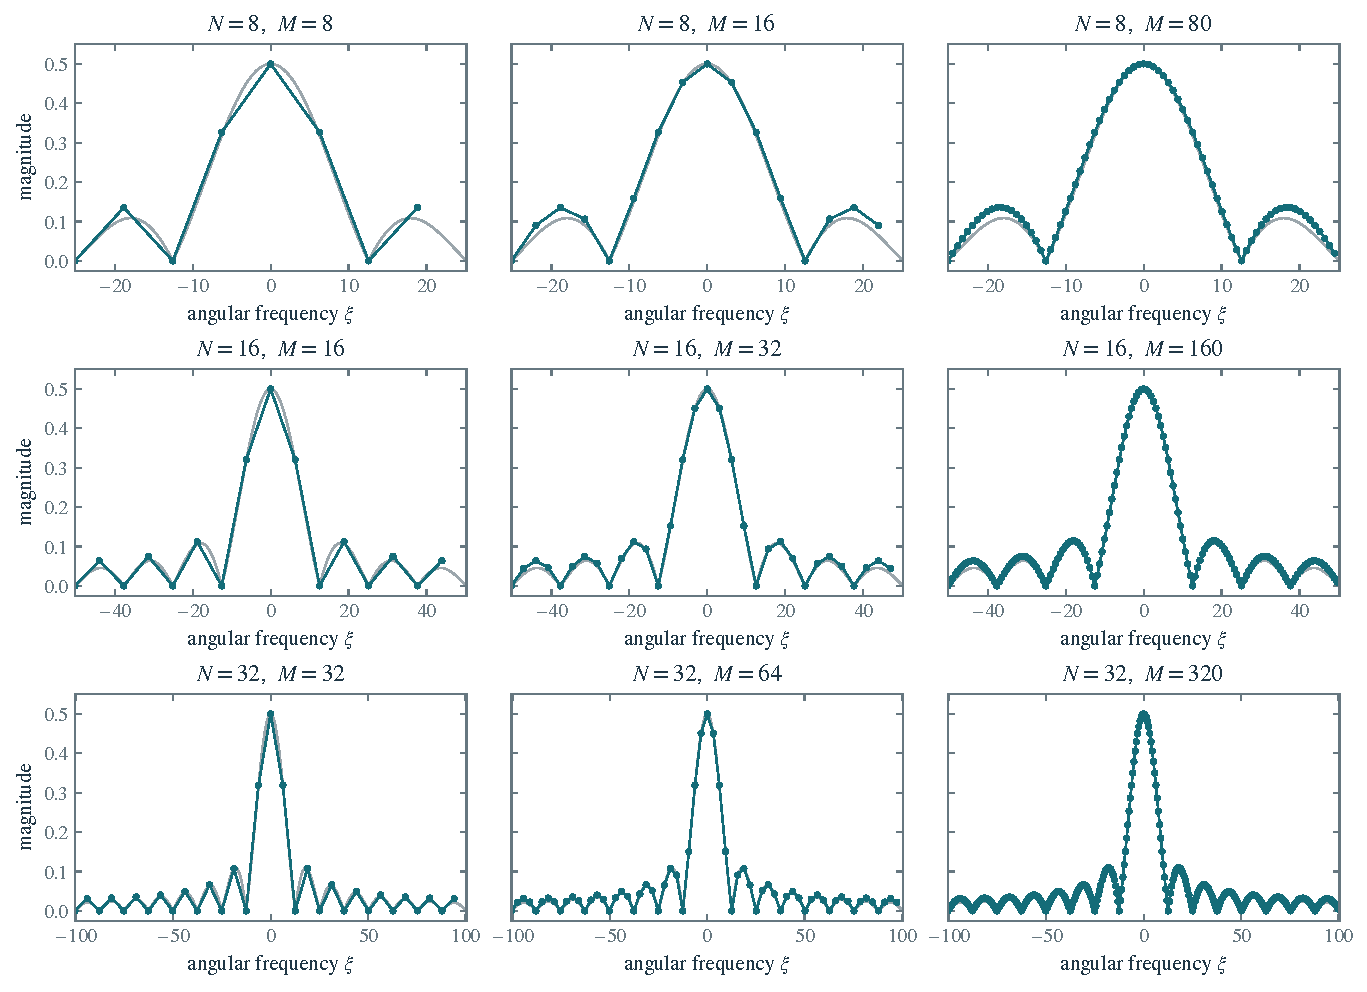
\includegraphics[width=1.0\linewidth]{figures/chapter-fourier-applications/sampling-and-padding/figure.pdf}
\caption{Sampling and zero padding for $f=\mathbf1_{[1/2,1)}$. Rows change the number $N$ of measured samples; columns change only the padded length $M$. The DFT magnitudes include the quadrature factor $1/N$; the faint curve is the continuous-transform magnitude.}
\label{fig-calcul-approach-tf}
\end{figure}
Exercise~\ref{exo-creation-low-pass-filter} applies the same distinction to
frequency responses.

\subsection{Time--frequency duality}
\label{sect2-duality-time-frequency}\index{Uncertainty!principle}
Concentration in time and concentration in frequency constrain one another.
We focus on compact support, where the obstruction is absolute and
connects frequency localization with analyticity.
\begin{prop}
\label{prop-trans-fourier-support-compact}\index{Support!compact}
A nonzero function $f\in L^2(\RR)$ and its Fourier transform cannot both
have compact support.
\end{prop}
Exercise~\ref{exo-transforme-sup-comp} proves this by showing that a
band-limited function extends to an entire function. In the finite setting,
all supports are finite, so the appropriate analogue is the support-size
uncertainty inequality. For example, the DFT of $\delta_0$ is the constant
vector $1$: a single time sample occupies every frequency.

\section{Filtering}
\label{sect1-filtering}
Convolution models linear filtering that treats each location in the same
way. Its Fourier representation lets us design the response frequency by
frequency, while the convolution kernel describes its local action.

\subsection{Linear filters}
\label{sec2-linear-filters}\label{notation-53}

A translation-invariant filter is specified by how it combines shifted
copies of the input. We begin with finite kernels, where this operation is
well defined without convergence assumptions, and explain how to implement
it on finite data.

\index{Filter!linear}\index{Impulse!response}
For a finitely supported sequence $g$, define
\[
 \Phi^g(f)[n]=(f\star g)[n]=\sum_{k\in\ZZ}g[k]f[n-k].
\]
This sum is well defined for every sequence $f$. The kernel $g$ is the
\emph{impulse response}, since $\Phi^g(\delta_0)=g$.
Its Fourier or $Z$ transform, rather than $g$ itself, is usually called the
transfer function. Finite support makes this a \emph{finite impulse response}
(FIR) filter. Infinite kernels require a convergence condition, discussed below.

For data supported in an interval of $N$ indices and a kernel supported in
an interval of $P$ indices, zero padding to at least $N+P-1$ permits exact
linear convolution by FFT. Store every index modulo the padded length,
including negative kernel indices, then extract and order the desired output.
For a short kernel, direct convolution can be cheaper than the FFT.

A useful example is a truncated discrete Gaussian,
\[
 g_\sigma[k]=\frac{e^{-k^2/(2\sigma^2)}}{\sum_{j=-r}^r e^{-j^2/(2\sigma^2)}},
 \quad -r\leq k\leq r,\qquad g_\sigma[k]=0\quad(|k|>r).
\]
It has unit sum and tends to $\delta_0$ as $\sigma\downarrow0$.
Increasing $\sigma$ spreads the averaging weights; the truncation radius
should be enlarged with $\sigma$ when an accurate Gaussian approximation is
wanted. Figure~\ref{fig-filter-smoothing} shows the resulting smoothing.
A sampled sequence has no differentiability class; the familiar smoothness
of continuous Gaussian convolution provides intuition rather than a literal
regularity theorem for a finite vector.
\begin{figure}[tbp]
\centering
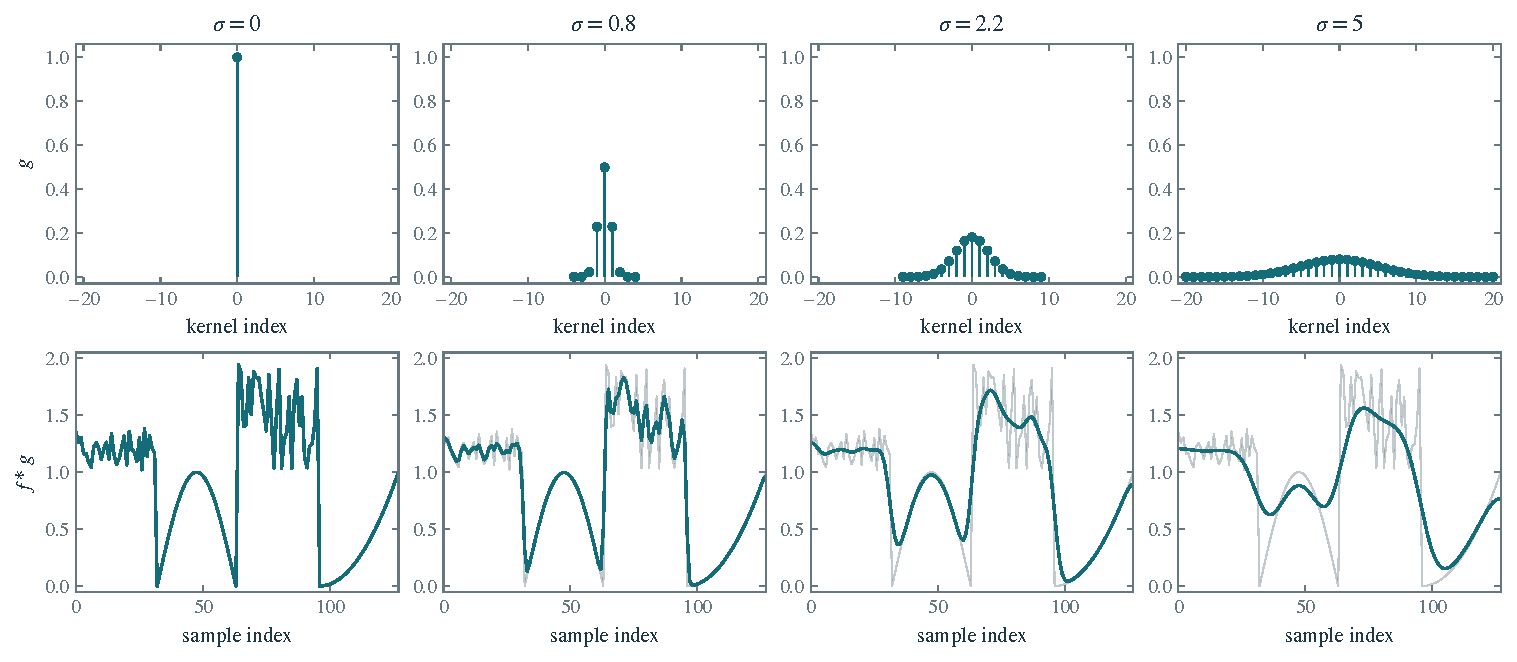
\includegraphics[width=1.0\linewidth]{figures/chapter-fourier-applications/gaussian-signal-smoothing/figure.pdf}
\caption{Gaussian kernels and their action on one fixed irregular signal. Widths are in sample units, and the signal is reflected at its endpoints. The first column is the exact identity kernel.}
\label{fig-filter-smoothing}
\end{figure}

\subsection{Responses and stability}
\label{sect2-responses-stability}

A kernel can be understood through its action on impulses, sinusoids, or
steps. These complementary descriptions guide filter design, while stability
asks whether bounded input can ever produce unbounded output.

\index{Frequency response}\index{Step!response}
Besides its impulse response, a filter has two useful descriptions:
\begin{itemize}
\item Its \emph{frequency response} is
$G(\omega)=\sum_k g[k]e^{-\imath k\omega}$. Indeed, filtering
$f[n]=e^{\imath\omega n}$ gives $G(\omega)e^{\imath\omega n}$.
The magnitude changes the amplitude and the argument changes the phase.
For an FIR filter, zero padding evaluates this trigonometric polynomial
on an arbitrarily fine frequency grid.
\item Its \emph{step response} is the output for $H[n]=1$ when $n\geq0$
and $H[n]=0$ otherwise:
$\Phi^g(H)[n]=\sum_{k\leq n}g[k]$.
It reveals how a sharp transition is blurred or accompanied by oscillations.
A finite vector of ones with zero extension contains two transitions,
so only the part unaffected by the second transition represents this response.
\end{itemize}
Figure~\ref{fig-diff-types-responses} compares impulse, frequency, and step
responses. A filter with nonzero negative-index coefficients is noncausal.
A narrow frequency transition typically requires a long or oscillatory
impulse response; neither description alone captures every design tradeoff.
\begin{figure}[tbp]
\centering
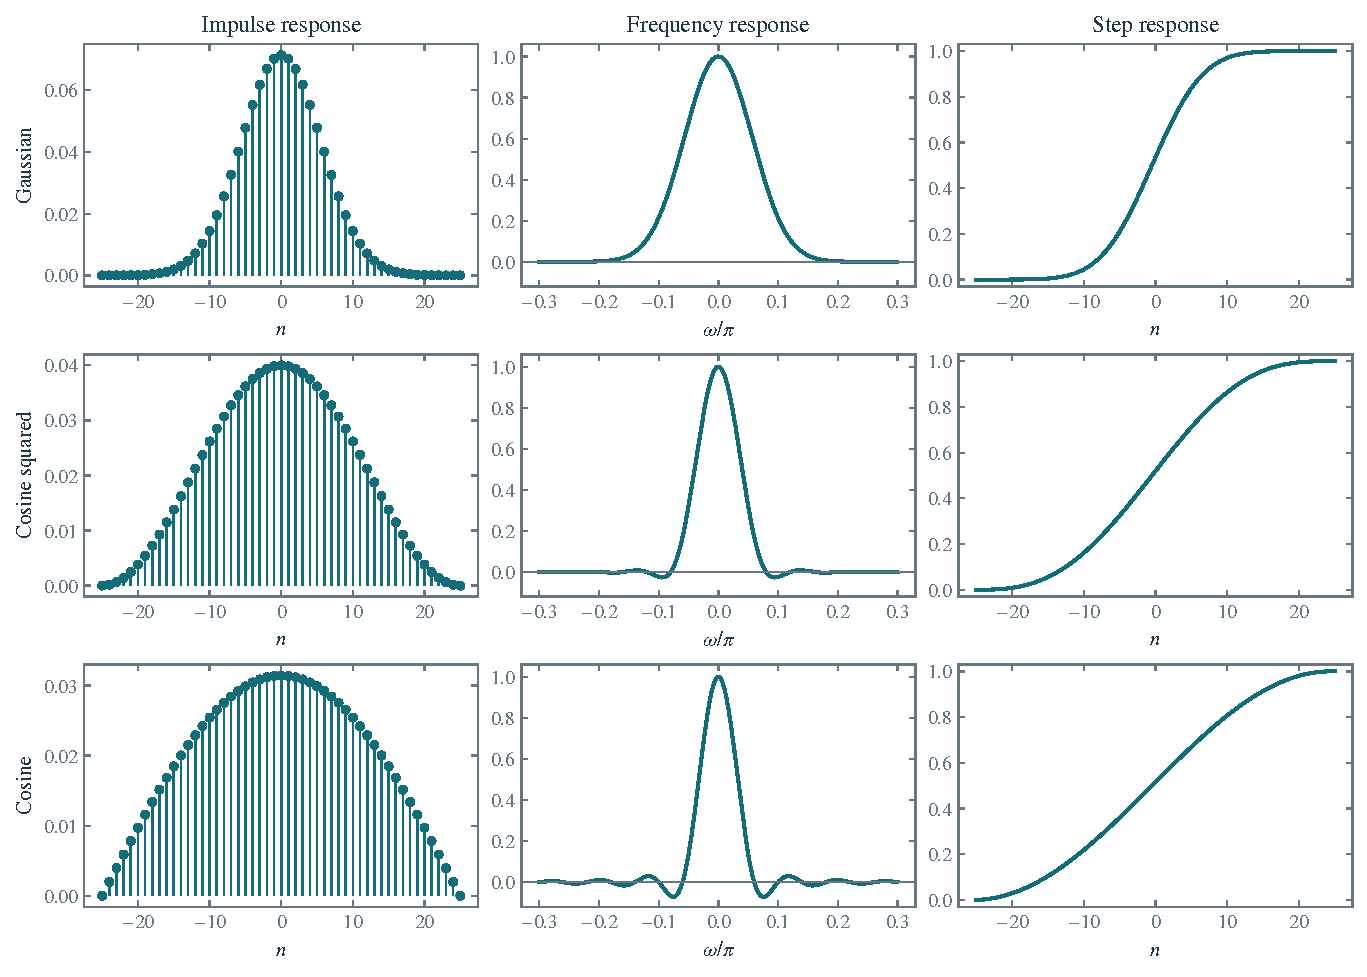
\includegraphics[width=1.0\linewidth]{figures/chapter-fourier-applications/filter-responses/figure.pdf}
\caption{Impulse, frequency, and step responses of three unit-sum symmetric FIR kernels. The frequency plots show a neighborhood of zero; the step responses are cumulative sums of the impulse responses.}
\label{fig-diff-types-responses}
\end{figure}

\statementintro{To control a filter's response to arbitrary bounded data, we use an operator
notion of stability.}

\begin{defn}[Bounded-input bounded-output stability]
\label{notation-54}\index{Stability}
A convolution filter is stable if it defines a bounded operator on
$\ell^\infty(\ZZ)$.
\end{defn}
The precise criterion is $g\in\ell^1(\ZZ)$. Sufficiency follows from
\[
 \|\Phi^g(f)\|_\infty\leq\|g\|_1\|f\|_\infty.
\]
For necessity, choose $f[-k]=\ol{g[k]}/|g[k]|$ when $g[k]\ne0$ and zero
otherwise. The convolution at zero is then $\sum_k|g[k]|$.
Equivalently, finitely supported truncations of this input show that a
uniform operator bound forces these partial sums to remain bounded.
The same test proves $\|\Phi^g\|_{\infty\to\infty}=\|g\|_1$.
Every FIR filter is stable; recursive filters need not be.
Section~\ref{sect2-application-trans-z-filters} returns to this distinction.

\subsection{Image filtering}
\label{sect2-filtering-2d}

Smoothing an image trades noise reduction against the loss of fine detail.
We extend Gaussian filtering to two dimensions and make the kernel scale and
boundary treatment part of the model.

\index{Filter!2D}\index{Image smoothing}
An image is an array of intensities, or several such arrays for color channels.
The two-dimensional version of the Gaussian kernel is
\[
 g_\sigma[k,l]=C_\sigma e^{-(k^2+l^2)/(2\sigma^2)},
 \qquad \sum_{k,l}g_\sigma[k,l]=1,
\]
with a specified finite support and normalizing constant $C_\sigma$.
Figure~\ref{fig-Gaussian-filter-2} compares kernels and the corresponding
smoothed images. Figure~\ref{fig-filter-2d} illustrates noise reduction.
Averaging attenuates noise but also blurs edges and fine texture.
Boundary handling is part of the model: zero extension darkens the border,
periodic extension joins opposite edges, and reflection avoids such a jump
when the image has no natural periodicity.
\begin{figure}[tbp]
\centering
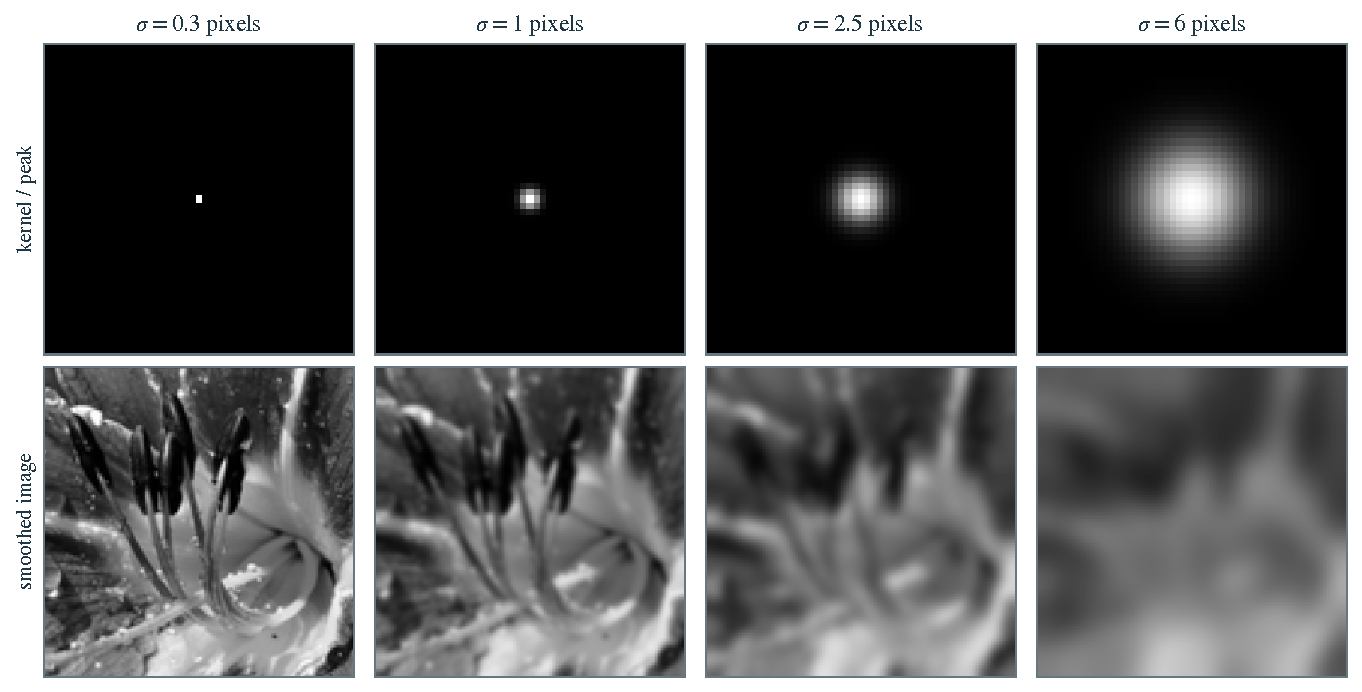
\includegraphics[width=1.0\linewidth]{figures/chapter-fourier-applications/gaussian-image-smoothing/figure.pdf}
\caption{Discrete Gaussian kernels (top) and smoothing of the flower image (bottom), with reflected boundaries. Each kernel is displayed relative to its own peak; all image panels share the grayscale range $[0,1]$.}
\label{fig-Gaussian-filter-2}
\end{figure}
\begin{figure}[tbp]
\centering
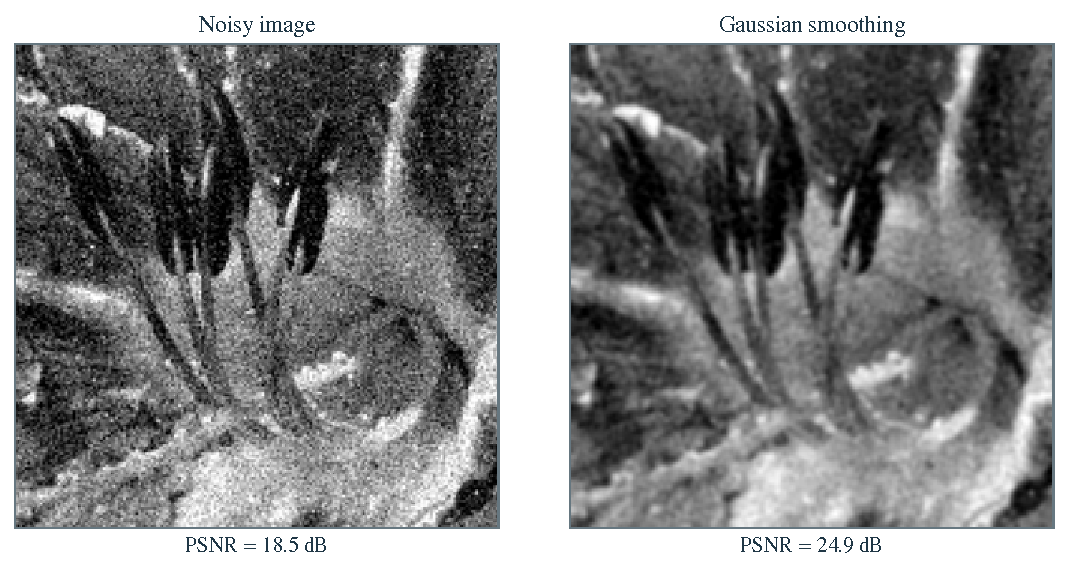
\includegraphics[width=1.0\linewidth]{figures/chapter-fourier-applications/image-denoising/figure.pdf}
\caption{A flower image corrupted by additive Gaussian noise of standard deviation $0.12$, and Gaussian smoothing with width $0.9$ pixels. The displayed PSNR values use the same clean reference; intensity clipping is for display only.}
\label{fig-filter-2d}
\end{figure}
Exercise~\ref{exo-correlation-2d} uses correlation to locate a smaller image
inside a larger one.

\section{Geometric aspects of filtering}
\label{sect1-aspect-geometriques}
A complex signal can also describe a polygon: its real and imaginary parts
are the two coordinates of a vertex. Circular convolution then acts directly
on shape, and Fourier coefficients expose its long-term behavior.

\subsection{Polygon filtering}
\label{sect2-filtering-polygons}

Repeated local averaging changes the shape of a polygon in ways that can be
read from a few Fourier multipliers. We describe the iteration in complex
coordinates and determine which frequencies persist, decay, or grow.

\index{Polygon}\index{Filter!of polygons}
Represent a closed polygon with $N$ ordered vertices by $\Pi\in\CC^N$,
joining $\Pi[j]$ to $\Pi[j+1\bmod N]$. For a circular filter $g$, let
\begin{equation}
\label{eq-filtering-polygons}
 \Pi^{(0)}=\Pi,\qquad \Pi^{(m+1)}=g*\Pi^{(m)}.
\end{equation}
Taking the DFT gives the exact formula
\[
 \widehat{\Pi^{(m)}}[k]=\wh g[k]^m\wh\Pi[k].
\]
Only \emph{active frequencies}, those with $\wh\Pi[k]\ne0$, affect the result.
If an active multiplier has modulus greater than one, the iterates are
unbounded. If every active multiplier has modulus at most one, they are
bounded. They converge precisely when each active multiplier either has
modulus strictly less than one or equals one; in that case
\[
 \widehat{\Pi^{(\infty)}}[k]=
 \begin{cases}\wh\Pi[k],&\wh g[k]=1,\\0,&\text{otherwise}.\end{cases}
\]
Active multipliers on the unit circle other than one prevent convergence.
When they are roots of unity, their surviving motion is periodic; decaying
modes generally make the full trajectory only \emph{asymptotically} periodic.
Figure~\ref{fig-filter-polygons-1} illustrates these cases.
\begin{figure}[tbp]
\centering
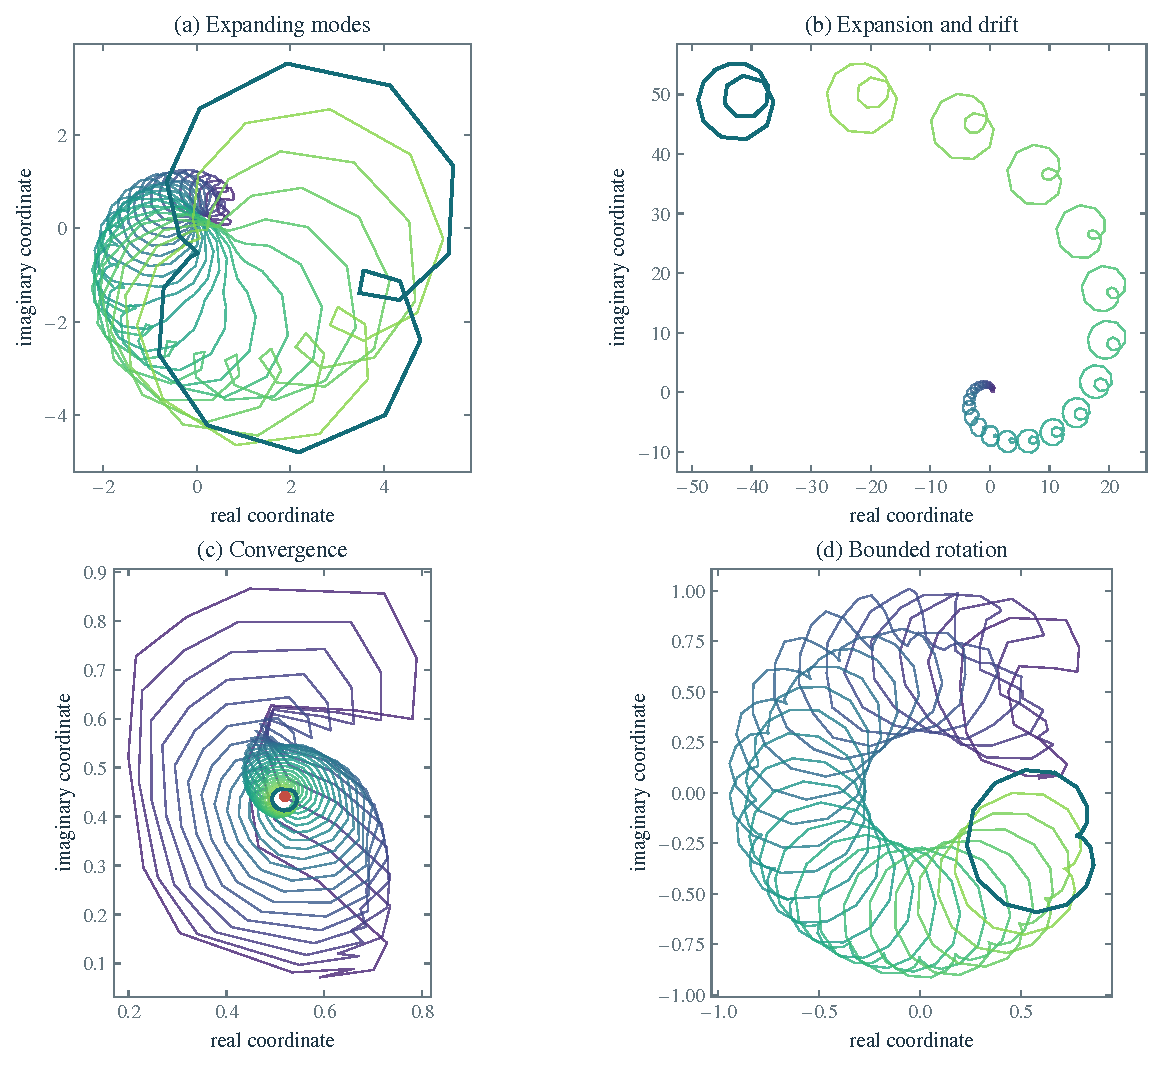
\includegraphics[width=1.0\linewidth]{figures/chapter-fourier-applications/polygon-iteration-regimes/figure.pdf}
\caption{Four regimes of polygon filtering. Curves progress from the initial polygon to later iterates. Expanding active multipliers cause divergence; unit-modulus phases can keep the trajectory bounded without convergence.}
\label{fig-filter-polygons-1}
\end{figure}

\statementintro{Repeatedly replacing adjacent vertices by their midpoint gives a simple
illustration of the spectral convergence criterion.}

\begin{exmp}[Successive midpoints]
\index{Center!of gravity}
For $g=(1/2,1/2,0,\ldots,0)$,
\[
 \Pi^{(1)}[j]=\tfrac12(\Pi[j]+\Pi[j-1]),\qquad
 \wh g[k]=e^{-\imath\pi k/N}\cos(\pi k/N).
\]
The multiplier is one at $k=0$ and has modulus less than one elsewhere.
The vertices therefore converge to their arithmetic mean
$c=N^{-1}\wh\Pi[0]$. This is the centroid of the vertices, which need not
be the area centroid of the enclosed region.
\end{exmp}

\statementintro{Retaining one nonconstant Fourier mode instead produces a nontrivial
limiting shape when that mode is present initially.}

\begin{exmp}[Keeping a single frequency]
If $\wh g[1]=1$ and $\wh g[k]=0.8$ for $k\ne1$, then
\[
 \Pi^{(\infty)}[j]=N^{-1}\wh\Pi[1]e^{2\pi\imath j/N}.
\]
For $\wh\Pi[1]\ne0$, the limit is a regular polygon centered at zero with
radius $|\wh\Pi[1]|/N$. If that coefficient vanishes, it collapses to zero.
\end{exmp}
\begin{figure}[tbp]
\centering
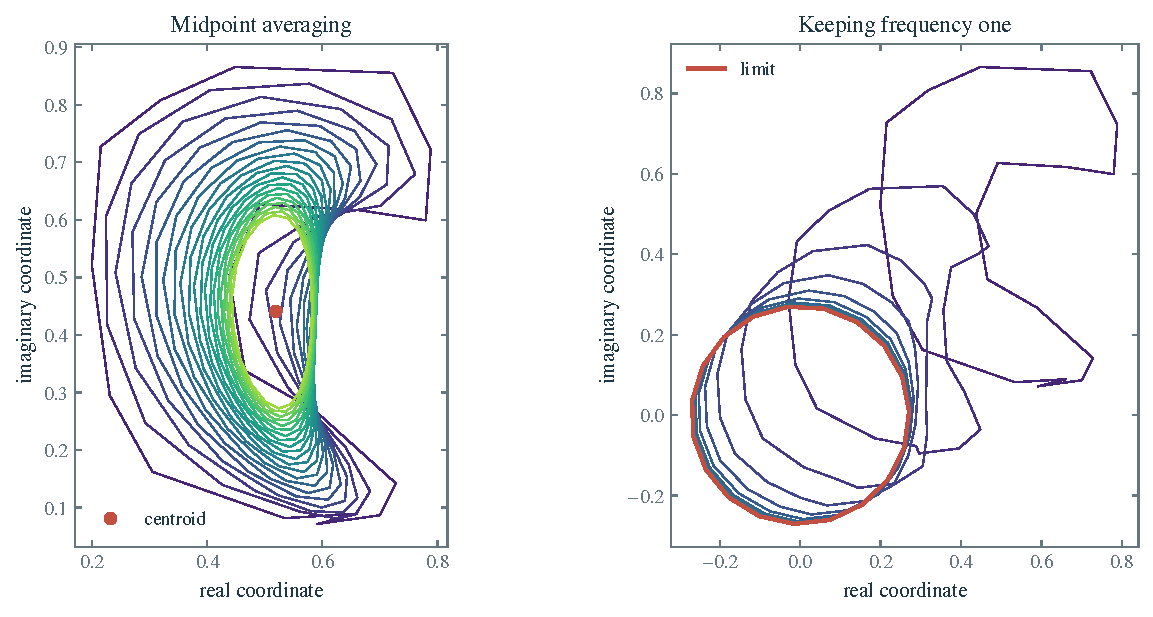
\includegraphics[width=1.0\linewidth]{figures/chapter-fourier-applications/polygon-filtering/figure.pdf}
\caption{Successive midpoint averaging converges to the vertex centroid (left). Keeping only frequency one produces a regular polygon of radius $|\widehat\Pi[1]|/N$ (right). Red marks indicate the limits.}
\label{fig-filter-polygons-2}
\end{figure}

\subsection{Polygonal inequalities}

Fourier coordinates relate a polygon's edge lengths, spread about its
center, and signed area. We use these expressions to prove geometric bounds
by comparing their contributions frequency by frequency.

\index{Inequality!polygonal}
The argument follows Terras~\cite{terras}. For $N\geq3$ and $c=N^{-1}\sum_j\Pi[j]$, set
\begin{align*}
 S(\Pi)&=\sum_j|\Pi[j+1]-\Pi[j]|^2,\\
 T(\Pi)&=\sum_j|\Pi[j]-c|^2,\\
 A(\Pi)&=\tfrac12\sum_j\imagp\bigl(\ol{\Pi[j]}\Pi[j+1]\bigr).
\end{align*}
The last expression is the signed area, including for self-intersecting
polygons, where it counts regions with their winding multiplicities.

\statementintro{Expressing these three quantities in Fourier coordinates gives two bounds
valid for every closed polygon.}

\begin{prop}
For every such polygon,
\[
 |A(\Pi)|\leq\tfrac12T(\Pi),\qquad
 4\sin^2(\pi/N)T(\Pi)\leq S(\Pi).
\]
\end{prop}
\begin{proof}
Let $z=\Pi-c$ and $Bz[j]=z[j+1]$. Translation leaves all three quantities
unchanged, $\wh z[0]=0$, and
$\widehat{Bz}[k]=e^{2\pi\imath k/N}\wh z[k]$. Plancherel gives
\begin{align*}
 T(\Pi)&=\frac1N\sum_{k=1}^{N-1}|\wh z[k]|^2,\\
 A(\Pi)&=\frac1{2N}\sum_{k=1}^{N-1}
             \sin(2\pi k/N)|\wh z[k]|^2,\\
 S(\Pi)&=\frac4N\sum_{k=1}^{N-1}
             \sin^2(\pi k/N)|\wh z[k]|^2.
\end{align*}
Use $|\sin(2\pi k/N)|\leq1$ in the second line and
$\sin^2(\pi k/N)\geq\sin^2(\pi/N)$ in the third.
\end{proof}

\subsection{Fourier descriptors}

For shape comparison, a useful descriptor should ignore translation, scale,
rotation, and the chosen starting vertex. We examine how these operations
change the Fourier coefficients and identify both the resulting invariants
and the information they discard.

\index{Fourier descriptor}\index{Pattern recognition}
A translation changes only $\wh\Pi[0]$. An orientation-preserving similarity
$z\mapsto a+bz$, with $b\ne0$, multiplies every other coefficient by $b$.
A cyclic change of starting vertex multiplies coefficient $k$ by a unit phase.
These observations motivate the real, nonnegative descriptor
\[
 \Dd(\Pi)=\left(\frac{|\wh\Pi[2]|}{|\wh\Pi[1]|},\ldots,
                    \frac{|\wh\Pi[N-1]|}{|\wh\Pi[1]|}\right),
 \qquad \wh\Pi[1]\ne0.
\]
It is invariant under these operations. A different nonzero reference
coefficient can be used when the first one vanishes, provided the same
choice is made in every comparison. Near a zero reference coefficient,
normalizing by the total nonconstant spectral energy is more robust.

For polygons with the same number of vertices, define the descriptor
\emph{discrepancy} by $d(\Pi_1,\Pi_2)=\|\Dd(\Pi_1)-\Dd(\Pi_2)\|_2$.
It is a pseudometric on this collection, not a distance that distinguishes
all shapes: arbitrary changes of individual Fourier phases preserve it.
It also does not automatically remove a reversal of vertex order or changes
in sampling density. Figure~\ref{fig-fourier-descriptors} illustrates a useful
comparison without claiming that equal descriptors imply equal shapes.
\begin{figure}[tbp]
\centering
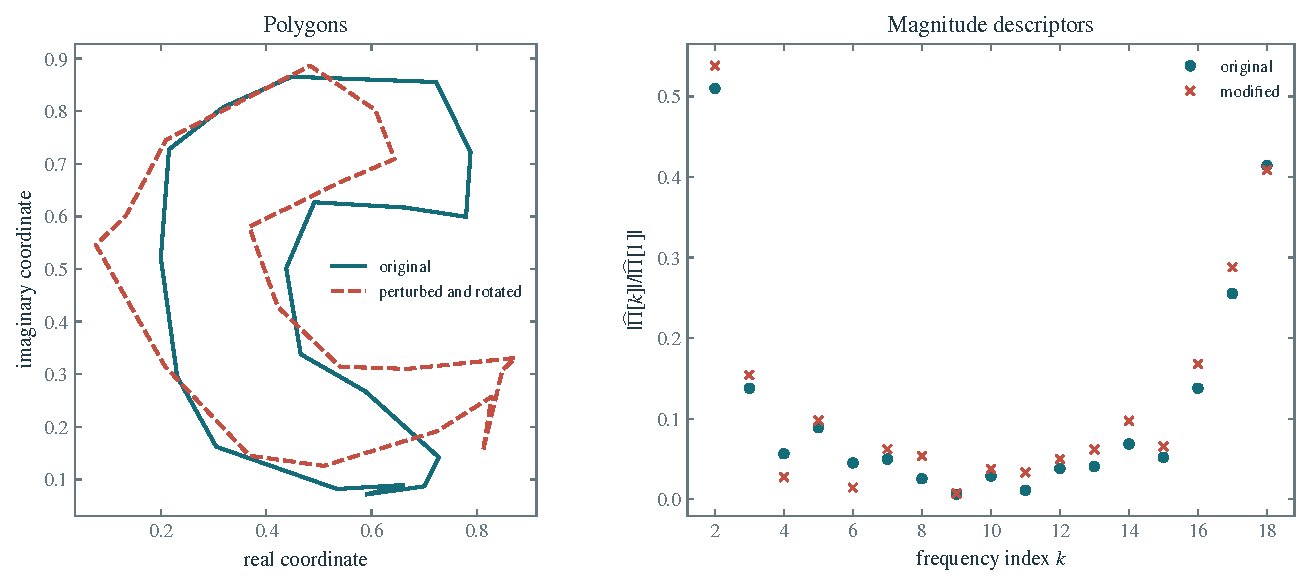
\includegraphics[width=1.0\linewidth]{figures/chapter-fourier-applications/fourier-descriptors/figure.pdf}
\caption{A polygon and a perturbed, rotated version, with their magnitude-based Fourier descriptors. The perturbation changes the descriptor; the rotation alone would leave it unchanged.}
\label{fig-fourier-descriptors}
\end{figure}

\section{Numerical solution of partial differential equations}
\label{sect1-resolution-edp}\index{Partial differential equation}
The Fourier transform converts differentiation in $x$ into multiplication by
$\imath\xi$. It therefore diagonalizes many constant-coefficient differential
operators. In a computation, the boundary conditions determine which Fourier
basis is appropriate: periodic exponentials for a circle, for example, or
sines for homogeneous Dirichlet conditions.

\subsection{Computing Fourier coefficients}
\label{sect2-calcul-coef-fourier}

A spectral solver needs Fourier coefficients of its initial data or source,
but a computation usually starts from samples. We examine the periodic
quadrature that connects the two and the aliasing error that remains.

For a continuous $T$-periodic function, let
\[
 c_k(f)=\frac1T\int_0^T f(t)e^{-2\pi\imath kt/T}\d t.
\]
Sampling $f[n]=f(nT/N)$ gives
\begin{equation}
\label{eq-lien-fft-calcul-coef-fourier}
 c_k(f)\approx\frac1N\sum_{n=0}^{N-1}f[n]e^{-2\pi\imath kn/N}
             =\frac1N\wh f[k\bmod N].
\end{equation}
For periodic data this is the composite trapezoidal rule, since the two
endpoint half-weights combine. Its accuracy can be far better than a
first-order rectangle estimate suggests. If the Fourier series is absolutely
convergent, substitution and discrete orthogonality give the exact aliasing
identity
\[
 \frac1N\wh f[k]=\sum_{\ell\in\ZZ}c_{k+\ell N}(f).
\]
The error is the sum of the aliased coefficients. Smoothness gives rapid
decay; analyticity in a strip gives exponential decay away from the sampling
limit. See Trefethen and Weideman~\cite{trefethen-weideman-trapezoidal}.
Increasing the sampling rate reduces this error. Zero padding alone does
not produce additional independent Fourier-series coefficients of $f$.

\subsection{The heat equation}
\label{sect2-resol-eq-heat}

Diffusion damps each Fourier mode at a rate determined by its frequency.
This diagonal evolution gives an explicit solution of the periodic heat
equation and a direct way to compute its smoothing effect.

\index{Equation!heat}
On the unit circle $S^1=\RR/\ZZ$, consider
\begin{equation}
\label{heat-eq}
 \partial_tu=\kappa\partial_{xx}u\quad(t>0),\qquad u(0,x)=f(x),
 \qquad\kappa>0.
\end{equation}
For continuous $f$, we seek a solution continuous up to $t=0$ and smooth
for $t>0$. Rescaling time reduces to $\kappa=1/2$, which we use here.
Writing $u(t,x)=\sum_n c_n(t)e^{2\pi\imath nx}$ and integrating twice by
parts gives
\[
 c_n'(t)=-2\pi^2n^2c_n(t),\qquad c_n(0)=c_n(f).
\]
Hence
\begin{equation}
\label{eq-solution-heat-equation}
 u(t,x)=\sum_{n\in\ZZ}c_n(f)e^{-2\pi^2n^2t}e^{2\pi\imath nx}.
\end{equation}
For $t\geq\epsilon>0$, this series and all its space and time derivatives
converge uniformly. Exercise~\ref{exo-unicite-eq-heat} proves uniqueness and
uniform convergence to continuous initial data as $t\downarrow0$.
Discontinuous data instead require an $L^2$ or pointwise interpretation;
uniform convergence to a discontinuous function is impossible.

The solution is convolution on the circle with the \emph{periodized}
Gaussian heat kernel. The mean is preserved and every nonconstant mode
decays, so the temperature becomes uniform. For the numerical solution,
replace $c_n(f)$ by $\wh f[n]/N$ and multiply the stored frequencies by
$e^{-2\pi^2n^2t}$. An inverse FFT evaluates the result on the original grid.
No time-stepping error is introduced in this spectral evolution; the spatial
sampling and truncation remain approximations.
The Python routines in Section~\ref{sect1-listing-heat} implement this method.
\begin{figure}[tbp]
\centering
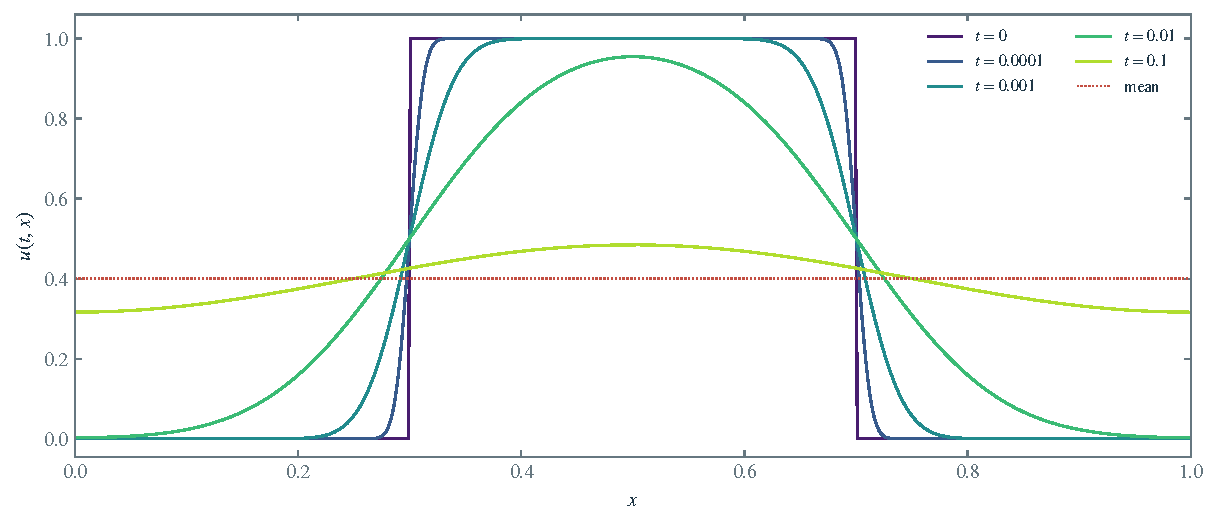
\includegraphics[width=1.0\linewidth]{figures/chapter-fourier-applications/heat-evolution/figure.pdf}
\caption{Spectral heat evolution of an interval indicator on the unit circle, with conductivity $\kappa=1/2$. The mean is preserved and the nonconstant Fourier modes decay.}
\label{fig-eq-heat-evolution}
\end{figure}
Heat evolution is one particular family of low-pass filters. A general
symmetric smoothing filter need not equal heat evolution at any time.

\subsection{The Poisson equation with Dirichlet data}
\label{sect2-resol-eq-Poisson}

Prescribed boundary values change the basis needed to solve a Poisson
problem. We discretize the equation on a square and use odd extensions to
recover an FFT-based solver that respects the Dirichlet conditions.

\index{Poisson's equation}
On the square, consider
\begin{equation}
\label{eq-fish}
 \Delta u=\partial_{xx}u+\partial_{yy}u=f\quad\text{in }(0,1)^2,
 \qquad u=b\quad\text{on }\partial[0,1]^2.
\end{equation}
The boundary values are prescribed and agree at the corners.
Poisson's equation models, among other problems, a deflected membrane or an
electrostatic potential, with physical constants and signs incorporated into
$f$. When $f=0$, the solution is harmonic.

Let $h=1/N$ and $U_{ij}\approx u(ih,jh)$ for $0\leq i,j\leq N$.
At the interior points use the five-point stencil
\begin{equation}
\label{eq-poisson-discretise}
 \frac{U_{i-1,j}+U_{i+1,j}+U_{i,j-1}+U_{i,j+1}-4U_{ij}}{h^2}=F_{ij},
 \qquad F_{ij}=f(ih,jh).
\end{equation}
This is a second-order consistent approximation when $u$ has four continuous
spatial derivatives. Its boundary values are fixed, so it is \emph{not} a
circular convolution on the original square.

Move each boundary contribution to the right-hand side. For $1\leq i,j<N$,
\begin{align*}
 \wt F_{ij}=F_{ij}-h^{-2}\bigl(&\mathbf1_{i=1}b_{0j}
 +\mathbf1_{i=N-1}b_{Nj}\\
 &+\mathbf1_{j=1}b_{i0}+\mathbf1_{j=N-1}b_{iN}\bigr).
\end{align*}
The unknown interior array now satisfies the same stencil with zero boundary
values. Extend it, and $\wt F$, oddly across each boundary and periodically
with period $2N$ in each coordinate. Denote the extensions by $U^o,F^o$.
For example, $F^o_{-i,j}=-F^o_{i,j}$ and
$F^o_{i,-j}=-F^o_{i,j}$; values on $i=0,N$ or $j=0,N$ vanish.
On the doubled grid the equation is exactly $\Phi*U^o=F^o$, with
\begin{equation}
\label{eq-filter-eq-fish}
 \Phi[0,0]=-4h^{-2},\qquad
 \Phi[\pm1,0]=\Phi[0,\pm1]=h^{-2},
\end{equation}
and all other entries zero (indices are modulo $2N$).
The convolution equation also holds on the reflection axes, where opposite
neighbors cancel.

The symbol of this stencil is
\[
 \wh\Phi[k,l]=h^{-2}\bigl(2\cos(\pi k/N)+2\cos(\pi l/N)-4\bigr)
 =-4h^{-2}\bigl(\sin^2(\pi k/(2N))+\sin^2(\pi l/(2N))\bigr).
\]
Thus, except at $(k,l)=(0,0)$,
\[
 \widehat{U^o}[k,l]=-
 \frac{h^2\widehat{F^o}[k,l]}{4\bigl(\sin^2(\pi k/(2N))+\sin^2(\pi l/(2N))\bigr)}.
\]
The zero mode is set to zero because an odd array has zero mean.
All other denominators are positive. The inverse FFT recovers $U^o$;
retain its interior on the original square and restore the prescribed boundary.
Equivalently, a discrete sine transform works directly on the interior array;
Exercise~\ref{exo-formulation-matrix-fish} proves the equivalence.

Section~\ref{sect1-listing-fish} implements the solver. For validation, choose
$u(x,y)=e^{xy}$, so $f=(x^2+y^2)e^{xy}$, and prescribe its boundary values.
Figure~\ref{fig-eq-fish} shows this case; Figure~\ref{fig-eq-Poisson-modif}
changes two edges while keeping compatible corners. For $u=x^2+y^2$, the
stencil gives $\Delta u=4$ exactly, so the computed nodal solution agrees
up to roundoff. In fact, centered second differences are exact for polynomials
of degree at most three; this does not make them exact for general smooth data.
\begin{figure}[tbp]
\begin{minipage}[t]{.485\linewidth}
\centering
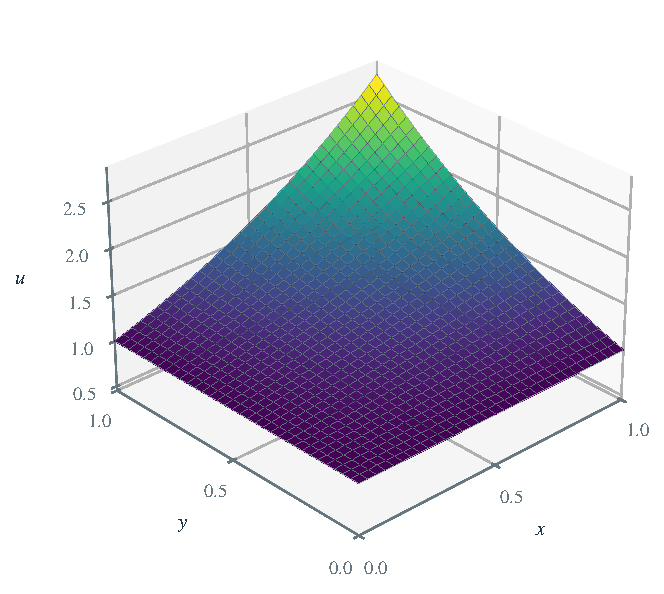
\includegraphics[width=1.0\linewidth]{figures/chapter-fourier-applications/poisson-reference/figure.pdf}
\caption{Dirichlet Poisson solution with reference $u(x,y)=e^{xy}$, on a grid with $N=32$ intervals per axis.}
\label{fig-eq-fish}
\end{minipage}\hfill
\begin{minipage}[t]{.485\linewidth}
\centering
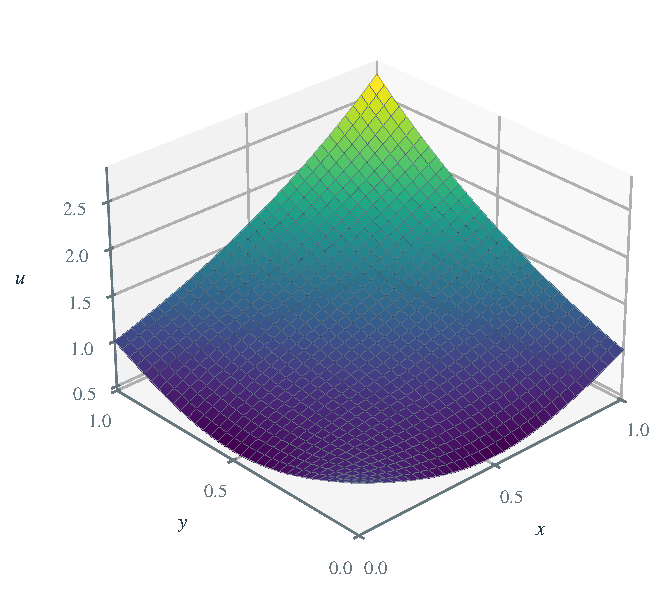
\includegraphics[width=1.0\linewidth]{figures/chapter-fourier-applications/poisson-modified-boundary/figure.pdf}
\caption{The same source with boundary values lowered by $0.45\sin(\pi s)$ on $x=0$ and $y=0$. All four corner values remain compatible.}
\label{fig-eq-Poisson-modif}
\end{minipage}
\end{figure}

\section{Fast products}
\label{sect1-calculations-products}
Convolution also describes polynomial multiplication. The FFT therefore
connects numerical signal processing to algebra and fast integer arithmetic;
Bailey~\cite{bailey-pi} gives historical examples involving high-precision
computation.

\subsection{Evaluation and interpolation}
\label{sect2-presentation-theoretical}

Polynomial multiplication is easy when polynomials are represented by their
values at suitable nodes. Evaluation and interpolation provide the change of
coordinates, with quotient algebras explaining exactly which product is
recovered.

\index{Polynomial!evaluation}
Choose \emph{distinct} points $\xi_0,\ldots,\xi_{M-1}$ and set
$Q(X)=\prod_{j=0}^{M-1}(X-\xi_j)$. Evaluation induces an algebra isomorphism
\[
 \Phi:\CC[X]/(Q)\longrightarrow\CC^M,
 \qquad [P]\longmapsto(P(\xi_0),\ldots,P(\xi_{M-1})),
\]
where the target uses coordinatewise multiplication. Its kernel before
passing to the quotient is $(Q)$: a polynomial vanishes at all the distinct
points if and only if their linear factors divide it. This is also the
Chinese remainder theorem for the pairwise coprime ideals $(X-\xi_j)$.
If points repeat, the kernel is generated by the product over the
\emph{distinct} points, and ordinary evaluations no longer give this isomorphism.

To multiply two polynomials modulo $Q$, evaluate both, multiply their values,
then interpolate. The multiplication of values costs $O(M)$ operations;
the usefulness of the method depends on the cost of the two changes of
representation. Roots of unity make these changes fast.

\subsection{Multiplication modulo \texorpdfstring{$X^N-1$}{X\^N-1}}
\label{sect2-multiplication-polynomials-modulo-xn-1}

Roots of unity make both evaluation and interpolation fast through the DFT.
The resulting product is naturally taken modulo $X^N-1$, so its coefficients
wrap around just as in circular convolution.

\index{Polynomial!multiplication}
For $\xi_k=e^{-2\pi\imath k/N}$, evaluation of a polynomial
$P=\sum_{j=0}^{N-1}P_jX^j$ is exactly the DFT of its coefficient vector.
Since $\prod_k(X-\xi_k)=X^N-1$, we obtain
\begin{equation}
\label{eq-prod-cyclic-polynomial}
 (PQ)\bmod(X^N-1)=\Ff^{-1}\bigl(\Ff(P)\cdot\Ff(Q)\bigr).
\end{equation}
The equality identifies a polynomial with its coefficient vector; on the
right, multiplication is entrywise. In coefficient form the same operation
is circular convolution. Figure~\ref{fig-convolution-polynomial} uses
$P=1+2X+X^3-X^4+X^5$ and $Q=X-X^2+2X^3+2X^5$.
Padding to length eleven preserves their degree-ten product without wraparound.
\begin{figure}[tbp]
\centering
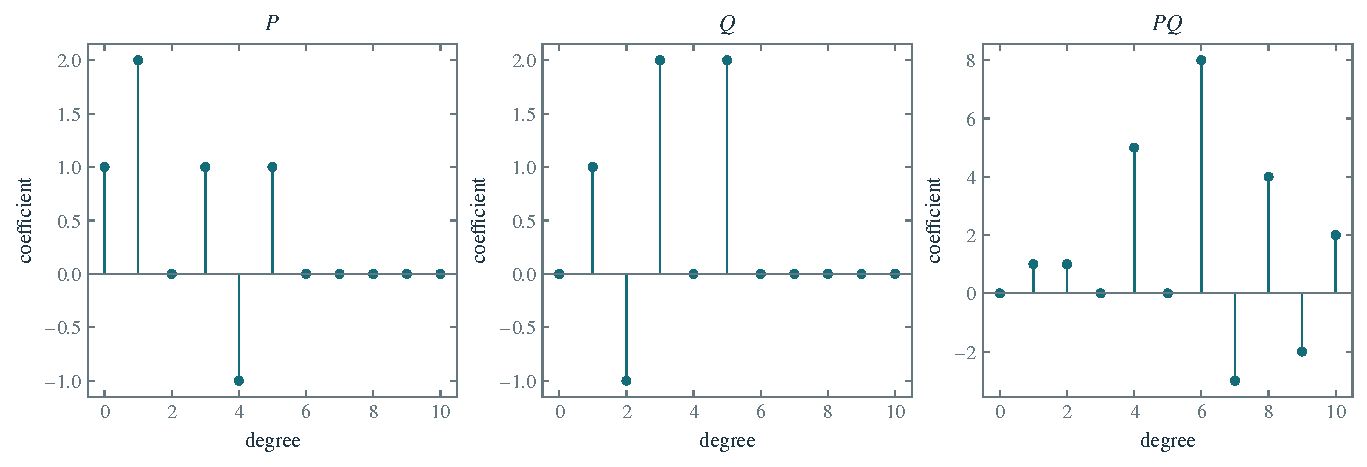
\includegraphics[width=1.0\linewidth]{figures/chapter-fourier-applications/polynomial-convolution/figure.pdf}
\caption{Coefficient vectors of $P$, $Q$, and their product. Length-eleven FFT convolution agrees with the ordinary degree-ten polynomial product.}
\label{fig-convolution-polynomial}
\end{figure}

For general distinct interpolation nodes, the Lagrange basis is
\[
 L_i(X)=\prod_{j\ne i}\frac{X-\xi_j}{\xi_i-\xi_j},\qquad
 P(X)=\sum_i P(\xi_i)L_i(X).
\]
Both products exclude $j=i$. Stable evaluation can use the barycentric
form of this formula; divided differences provide another representation.
The conditioning depends strongly on the nodes, as the Chebyshev example
in Chapter~\ref{chap-tfd} illustrates.

\subsection{Ordinary polynomial multiplication}
\label{sect2-multiplication-polynomials}

To recover the full polynomial product, the transform must leave room for
every output coefficient. Zero padding prevents reduction modulo the
transform polynomial from mixing those coefficients.

If $\deg P,\deg Q\leq N-1$, then $\deg(PQ)\leq2N-2$ and
\begin{equation}
\label{eq-product-polynomials}
 (PQ)_n=\sum_kP_kQ_{n-k},\qquad 0\leq n\leq2N-2,
\end{equation}
where coefficients outside $0,\ldots,N-1$ are zero.
Pad both coefficient vectors to a transform length $M\geq2N-1$.
Reduction modulo $X^M-1$ then has no effect on their product, so circular
convolution gives ordinary multiplication. A convenient smooth transform
length yields an $O(M\log M)$ algorithm.

\subsection{Multiplication of large integers}
\label{sect2-multiplication-integers}

Integer multiplication has the same convolution structure as polynomial
multiplication, followed by carry propagation. We explain this connection
while distinguishing exact digit arithmetic from the rounding required by a
floating-point FFT.

\index{Integer!multiplication}
Write nonnegative integers in base $b\geq2$ as
\[
 a=\sum_{j=0}^{N-1}a_jb^j,\qquad 0\leq a_j<b.
\]
Their product is obtained by convolving the digit vectors and propagating
carries. If a temporary coefficient is $c_j$, replace it by its remainder
modulo $b$ and add $\lfloor c_j/b\rfloor$ to the next position, continuing
until the final carry vanishes. Section~\ref{sect1-listing-mult-integers}
implements these steps in Python.

A floating-point FFT only approximates the convolution. Rounding recovers
the integer coefficients when every error is strictly less than $1/2$;
this needs a precision bound or independent verification, not merely a
small observed distance to an integer. The examples check against Python's
exact integers. Chapter~\ref{chap-extension-finite-field-values} develops
transforms over finite fields and rings, which permit exact modular arithmetic.

\section{Exercises}
\label{sect1-chap3-exercises}

These exercises connect the algebraic formulas with analytic proofs and
numerical implementations. We begin by justifying the compact-support
obstruction, then explore differential equations, image processing, and fast
arithmetic.

\statementintro{A compactly supported spectrum forces analyticity, which rules out a second
compact support in the original variable.}

\begin{exo}[Compact support and analyticity]
\label{exo-transforme-sup-comp}\index{Support!compact}
Let $f\in L^2(\RR)$ and suppose $\Supp(\wh f)\subset[-A,A]$.
Use Fourier inversion to construct a continuous representative of $f$ and
show that it is smooth. Express $f^{(n)}(t_0)$ as an integral, then expand
the exponential to prove that
\[
 f(t)=\sum_{n=0}^\infty\frac{f^{(n)}(t_0)}{n!}(t-t_0)^n
\]
for every real $t$. Justify the exchange of summation and integration.
Deduce that a nonzero $f$ cannot vanish on an open interval, and prove
Proposition~\ref{prop-trans-fourier-support-compact}.
\end{exo}

\statementintro{Fourier modes reveal when a time-stepping scheme for diffusion is stable and
how strongly it damps each spatial frequency.}

\begin{exo}[Finite differences for the heat equation]
\label{exo-resol-eq-heat-diff-finies}\index{Equation!heat}
On $S^1=\RR/\ZZ$, consider the conductivity-one equation
\begin{equation}
\label{eq-heat-exo}
 \partial_tu=\partial_{xx}u,\qquad u(0,x)=f(x).
\end{equation}
Let $d=1/N$, let $h>0$ be the time step, and write
$u^m[k]\approx u(mh,kd)$, with indices modulo $N\geq3$.
\begin{enumerate}
\item Derive the explicit scheme, valid at \emph{every} index $0\leq k<N$,
\[
 u^{m+1}[k]=u^m[k]+s\bigl(u^m[k+1]+u^m[k-1]-2u^m[k]\bigr),
 \qquad s=h/d^2.
\]
\item Express one step as a circular convolution. Compare direct evaluation
of the three-point stencil with applying an FFT at every step. Write a Python
implementation. How can the FFT help if only the result after many steps is needed?
\item The scheme is stable if its powers are bounded for every initial vector.
Determine its Fourier multipliers and the exact condition on a fixed grid.
Show that $s\leq1/2$ is necessary and sufficient for even $N$, and sufficient
for every $N$. State the slightly different sharp bound for odd $N$.
\item For $0\leq\theta\leq1$, consider
\[
 u^{m+1}-u^m=A*\bigl(\theta u^{m+1}+(1-\theta)u^m\bigr),
 \qquad A[0]=-2s,\quad A[1]=A[-1]=s.
\]
Find the Fourier multiplier and characterize stability. Identify the values
of $\theta$ for which stability holds for every $s\geq0$.
\item Extend the method to a periodic square grid. Derive the two-dimensional
stability bound and implement the method by a two-dimensional FFT.
Explain why a stable method can still exhibit sign-changing temporal
oscillations of high-frequency modes.
\end{enumerate}
Figure~\ref{fig-eq-heat-finite-diff} compares explicit Euler, Crank--Nicolson,
and backward Euler at a common large time step. The first is unstable;
the second is stable but damps the highest frequencies poorly at that step;
the third damps them strongly. Temporal oscillation and instability are
not equivalent.
\begin{figure}[tbp]
\centering
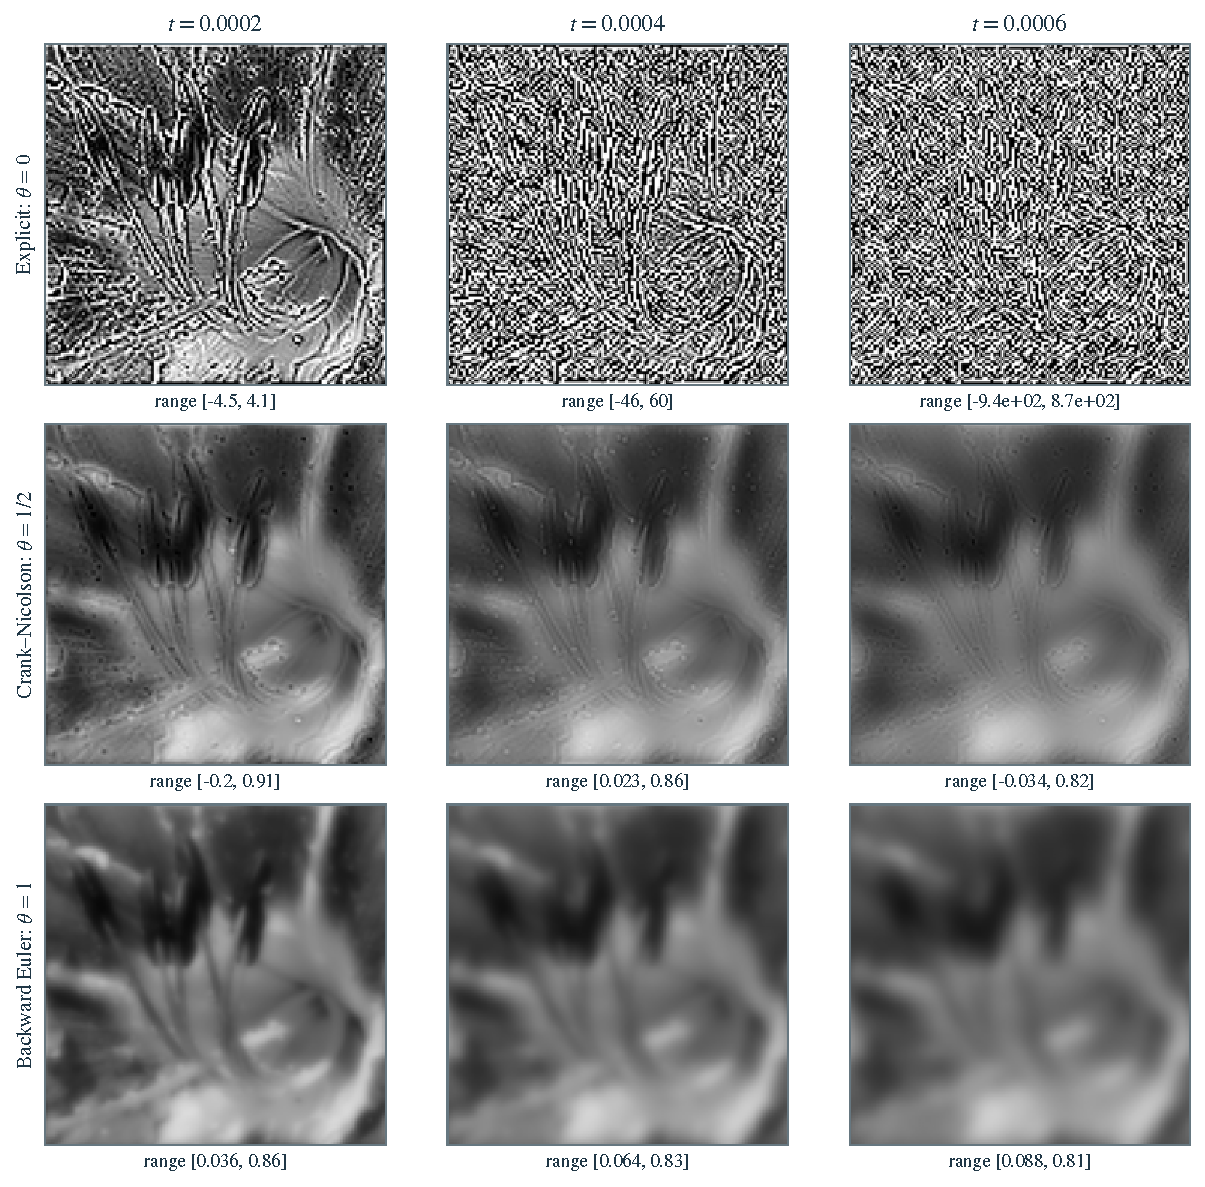
\includegraphics[width=1.0\linewidth]{figures/chapter-fourier-applications/heat-time-stepping/figure.pdf}
\caption{Three time steps for the same flower image, with $N=128$ and $h=0.0002$. Explicit Euler is unstable; Crank--Nicolson is stable but weakly damps high frequencies; backward Euler damps them strongly. All images use $[0,1]$, and each panel reports its actual value range.}
\label{fig-eq-heat-finite-diff}
\end{figure}
\end{exo}

\statementintro{The explicit Fourier solution also supports a proof of existence and
uniqueness for continuous initial data.}

\begin{exo}[Existence and uniqueness for the heat equation]
\label{exo-unicite-eq-heat}
Use the conductivity $\kappa=1/2$ of \eqref{heat-eq}, and suppose
$f\in C(S^1)$. This argument follows Dym and McKean~\cite{dym}.
\begin{enumerate}
\item Show that \eqref{eq-solution-heat-equation} equals
\[
 u(t,x)=\int_0^1p_t(x-y)f(y)\d y,\qquad
 p_t(x)=\sum_{n\in\ZZ}e^{-2\pi^2n^2t}e^{2\pi\imath nx}.
\]
Justify differentiation for $t>0$.
\item For $f\in C^2(S^1)$, prove $\|u(t,\cdot)-f\|_\infty\to0$
as $t\downarrow0$ using the decay of its Fourier coefficients.
\item Prove positivity for any real classical solution continuous up to
$t=0$: if $f\geq0$, then $u\geq0$. Apply a minimum argument to
$v(t,x)=e^{\beta t}u(t,x)$ with $\beta<0$. At a negative space-time
minimum $(t_1,x_1)$ with $t_1>0$, use
$0\geq v_t=\beta v+\tfrac12v_{xx}\geq\beta v>0$.
\item Deduce that $p_t\geq0$, that $\int_0^1p_t=1$, and that
$\|p_t*f\|_\infty\leq\|f\|_\infty$. Prove uniqueness among classical
solutions continuous up to their initial data, without assuming in advance
that every solution has the convolution representation.
\item Approximate a continuous $f$ uniformly by smooth periodic functions
to conclude $\|u(t,\cdot)-f\|_\infty\to0$.
\end{enumerate}
\end{exo}

\statementintro{The odd-extension construction extends coordinate by coordinate to a
three-dimensional Dirichlet problem.}

\begin{exo}[A three-dimensional Poisson problem]
\label{exo-potential-electric-3d}\index{Electric potential}
Generalize the Dirichlet solver of Section~\ref{sect2-resol-eq-Poisson} to
$\Delta u=f$ on the unit cube. Derive the seven-point stencil, transfer the
prescribed boundary values to the right-hand side, and extend the interior
array oddly in all three coordinates. Give the Fourier symbol and a Python
implementation of the extension. To visualize an electric potential, one
may plot its level surfaces $u(x,y,z)=\lambda$, rather than level surfaces
of the source $f$.
\end{exo}

\statementintro{The same solver can be understood through the eigenvectors of a tridiagonal
matrix, making its connection with sine transforms explicit.}

\begin{exo}[Matrix formulation of the Poisson solver]
\label{exo-formulation-matrix-fish}
This exercise relates the FFT construction to matrix diagonalization; see
Swarztrauber and Sweet~\cite{swarztrauber}.
Let $T=h^{-2}\operatorname{tridiag}(1,-2,1)$ have size $N-1$.
\begin{enumerate}
\item Show that the interior equation with zero boundary values is
$TU+UT=F$. Explain which coordinate each multiplication acts on.
\item With nonzero prescribed boundary values, derive
\begin{equation}
\label{eqn-exo-matrix-formulation-1}
 T\wt U+\wt UT=\wt F,
\end{equation}
where $\wt F$ includes the boundary corrections of the main text.
\item Show that $V_{ij}=\sin(\pi ij/N)$, $1\leq i,j<N$, diagonalizes $T$.
Find its eigenvalues $\lambda_j$, including the factor $h^{-2}$, and solve
the transformed equation entrywise.
\item Prove $V^TV=(N/2)I$, so $Q=\sqrt{2/N}V$ is orthogonal.
Relate multiplication by $V$ to the sine transform
$\Ss(x)[i]=\sum_{j=1}^{N-1}x[j]\sin(\pi ij/N)$.
\item Express $\Ss$ as a length-$2N$ DFT of an odd extension.
Give its inverse and its two-dimensional version, with all normalization
factors. Explain why this is equivalent to the doubled-grid solver.
\end{enumerate}
\end{exo}

\statementintro{A reproducible smoothing experiment must specify both the Gaussian kernel
and the treatment of image boundaries.}

\begin{exo}[Image smoothing]
\label{exo-lissage-image}\index{Image smoothing}
Implement Gaussian smoothing of a grayscale image. Specify the kernel
normalization, its truncation radius, and the boundary extension.
Verify that a constant image remains constant with reflection boundaries,
and compare the effect of several smoothing widths as in
Figure~\ref{fig-filter-2d}.
\end{exo}

\statementintro{Expanding a patch-matching error separates local energy from correlation and
shows when FFT correlation is an appropriate search tool.}

\begin{exo}[Correlation and template matching]
\label{exo-correlation-2d}\index{Correlation}
Let $f\in\RR^{N\times N}$ be an image and $g\in\RR^{P\times P}$ a template,
with $1\leq P\leq N$. Only consider positions $0\leq u,v\leq N-P$,
so that the entire template lies inside the image. Define
\[
 d(f,g)[u,v]^2=\sum_{i,j=0}^{P-1}\bigl(f[u+i,v+j]-g[i,j]\bigr)^2.
\]
\begin{enumerate}
\item\label{notation-55} Expand this expression using the local energy
$E_f[u,v]=\sum_{i,j}f[u+i,v+j]^2$ and the correlation
$\Corr(f,g)[u,v]=\sum_{i,j}f[u+i,v+j]g[i,j]$.
When does maximizing correlation minimize $d$?
\item Express correlation as linear convolution with a reflected template.
Explain the padding and output indices required for an FFT implementation.
\item\label{notation-56} Let $\mu_f[u,v]$ and $\mu_g$ be the patch and template
means. Define normalized correlation by
\[
 \rho[u,v]=
 \frac{\sum_{i,j}(f[u+i,v+j]-\mu_f[u,v])(g[i,j]-\mu_g)}
 {\sqrt{\sum_{i,j}(f[u+i,v+j]-\mu_f[u,v])^2}
  \sqrt{\sum_{i,j}(g[i,j]-\mu_g)^2}}.
\]
State when this expression is defined. Prove $|\rho|\leq1$, characterize
$\rho=1$, and describe its behavior under affine intensity changes.
\item Express the numerator as a correlation with the centered template.
For $k=1,2$, set $s_k[u,v]=\sum_{i,j=0}^{P-1}f[u+i,v+j]^k$.
With zero extension outside the image, establish the recurrence
\begin{align*}
 s_k[u,v]={}&s_k[u+1,v]+s_k[u,v+1]-s_k[u+1,v+1]\\
 &+f[u,v]^k+f[u+P,v+P]^k-f[u+P,v]^k-f[u,v+P]^k.
\end{align*}
Alternatively, derive a summed-area-table formula. Use these sums to compute
all patch variances in $O(N^2)$ work, then implement normalized correlation.
Do not assign a mathematically meaningful correlation to a constant patch.
\end{enumerate}
Figure~\ref{fig-correlation-2d} illustrates the distinction between raw and
normalized correlation. Lewis~\cite{lewis} discusses fast template matching.
\begin{figure}[tbp]
\centering
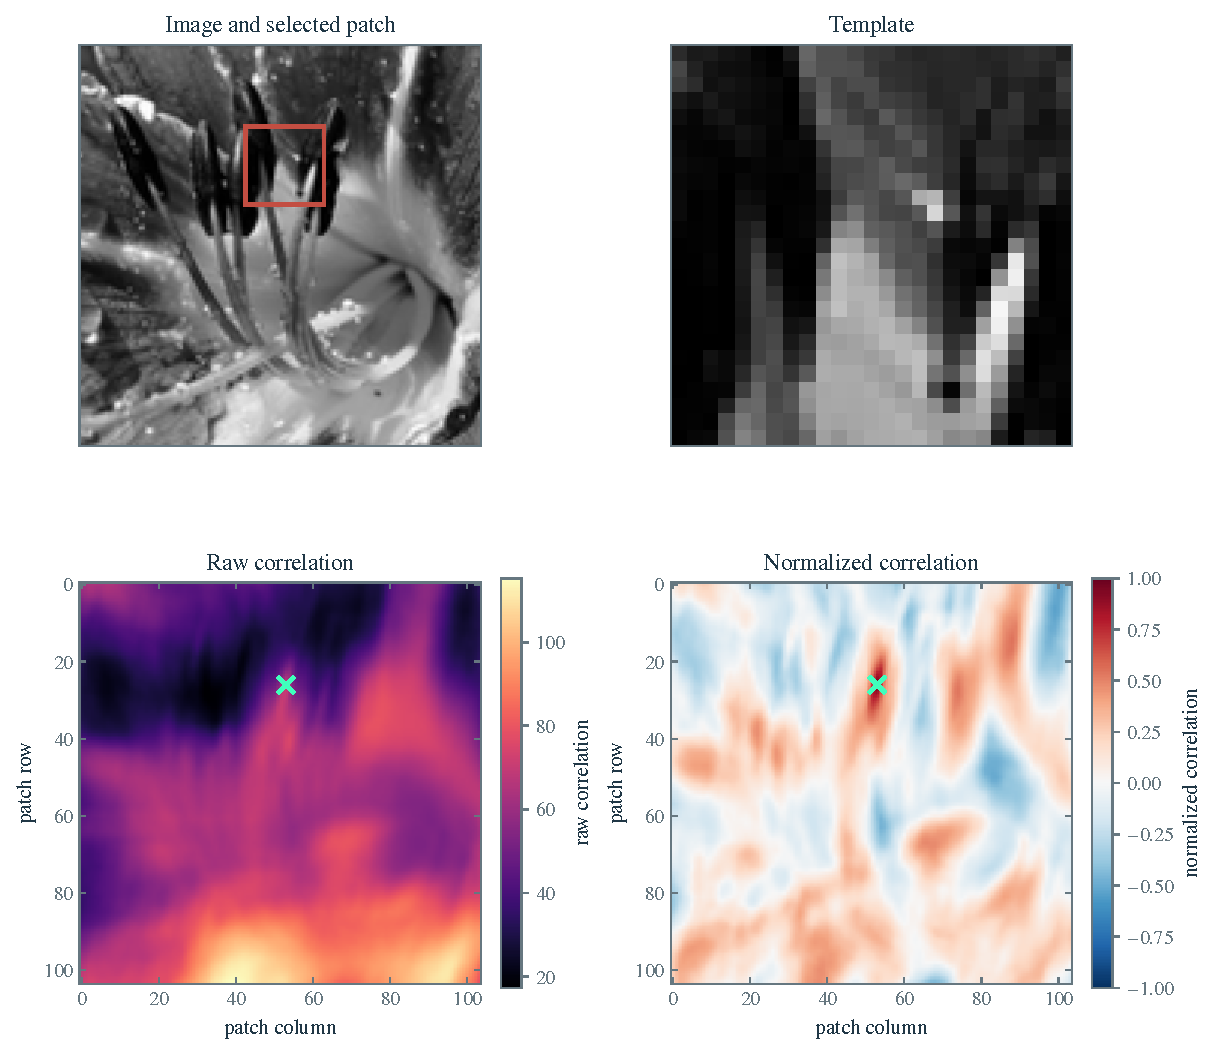
\includegraphics[width=1.0\linewidth]{figures/chapter-fourier-applications/template-matching/figure.pdf}
\caption{Template matching in the flower image. The red box identifies the extracted patch; crosses mark its location in the raw and normalized correlation maps. Only complete-template positions are included.}
\label{fig-correlation-2d}
\end{figure}
\end{exo}

\statementintro{Fractional translations implemented by Fourier phases can be combined into
shears and image rotations.}

\begin{exo}[Translation, shears, and rotation by FFT]
\label{exo-fft-rotation}\index{Rotation}\index{Translation}
Take an odd sample count $N$ in each coordinate. Interpret noninteger samples
through periodic trigonometric interpolation on the centered grid.
For a continuous image, define
\[
 T_vf(x,y)=f(x-v_1,y-v_2),\quad
 S_\lambda^{(x)}f(x,y)=f(x-\lambda y,y),\quad
 S_\lambda^{(y)}f(x,y)=f(x,y-\lambda x).
\]
\begin{enumerate}
\item Derive the Fourier phase multiplier for a translation. Apply one-dimensional
translations along rows or columns to implement each shear.
Why does the use of signed frequency indices matter for fractional shifts?
\item For $|\theta|<\pi$, prove
\[
 \begin{pmatrix}\cos\theta&-\sin\theta\\\sin\theta&\cos\theta\end{pmatrix}
 =\begin{pmatrix}1&-\tan(\theta/2)\\0&1\end{pmatrix}
  \begin{pmatrix}1&0\\\sin\theta&1\end{pmatrix}
  \begin{pmatrix}1&-\tan(\theta/2)\\0&1\end{pmatrix}.
\]
Deduce a three-shear algorithm for the pullback rotation
$R_\theta f(z)=f(\mathcal R_{-\theta}z)$.
\item Explain how centering and padding reduce wraparound artifacts. Show
that each discrete shear is unitary and invertible when complex values are
retained. Why does the finite-grid three-shear rotation generally fail the
exact composition law $R_\alpha R_\beta=R_{\alpha+\beta}$?
Discuss large angles and the need to avoid $\tan(\theta/2)$ near its poles.
\end{enumerate}
\begin{figure}[tbp]
\centering
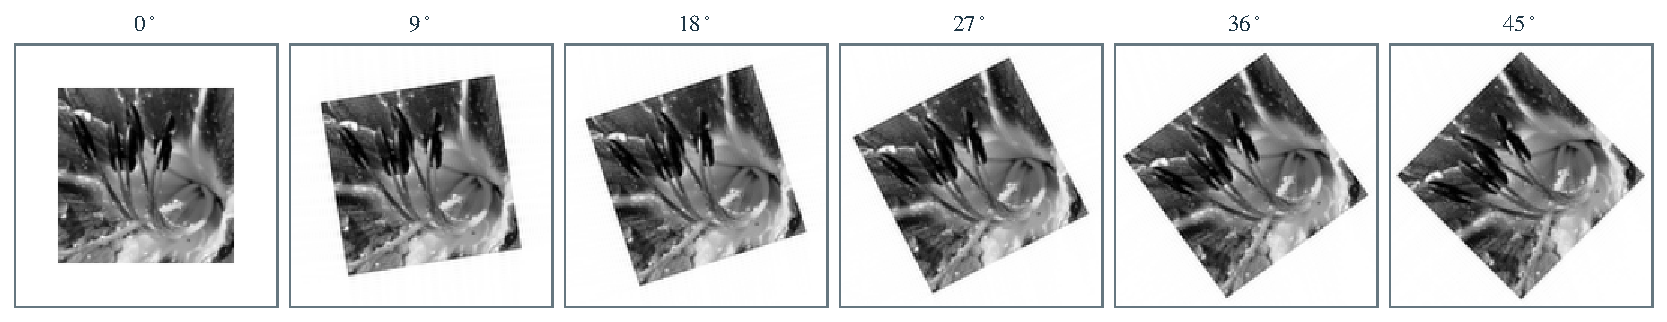
\includegraphics[width=1.0\linewidth]{figures/chapter-fourier-applications/fourier-image-rotation/figure.pdf}
\caption{Rotations of the flower image by three Fourier shears. The odd grid avoids a Nyquist ambiguity; a white margin limits wraparound. Cropping and intensity clipping are applied only to the displayed results.}
\label{fig-fft-rotation}
\end{figure}
\end{exo}

\statementintro{Designing a filter in frequency coordinates exposes the tradeoff between a
sharp cutoff and localization of its impulse response.}

\begin{exo}[Designing a low-pass filter]
\label{exo-creation-low-pass-filter}\index{Filter!low-pass}
Use an odd length $N$ and signed frequencies $\omega_k=2\pi k/N$.
\begin{enumerate}
\item Construct a real circular kernel whose frequency response is one for
$|\omega_k|<\pi/2$ and zero for $|\omega_k|>\pi/2$.
Specify a half-value at a cutoff frequency if it is present.
\item Regard the centered kernel as a finite sequence on $\ZZ$ and plot its
frequency response on a fine grid by zero padding. Compare the resulting
trigonometric polynomial with the prescribed samples.
\item Replace the sharp cutoff by a raised-cosine transition of width
$\epsilon\pi$ centered at each cutoff, for $0\leq\epsilon\leq1$.
Compare the impulse responses and the frequency-domain oscillations.
\end{enumerate}
\begin{figure}[tbp]
\centering
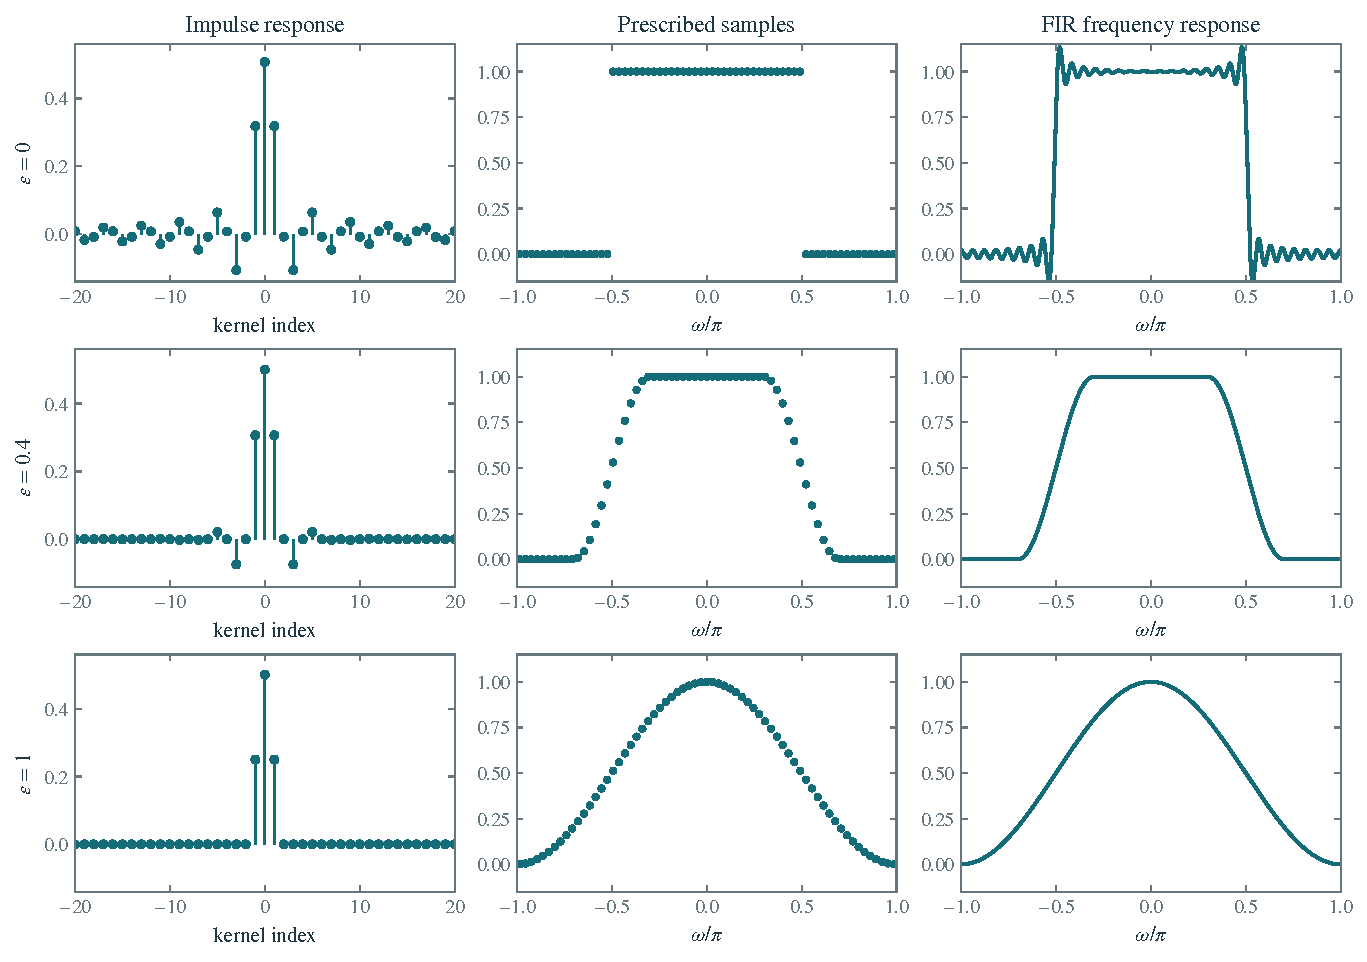
\includegraphics[width=1.0\linewidth]{figures/chapter-fourier-applications/low-pass-filters/figure.pdf}
\caption{Low-pass filters with increasingly wide raised-cosine transitions. The columns show the centered impulse response, the prescribed DFT samples, and the densely sampled FIR frequency response.}
\label{fig-low-pass-filter}
\end{figure}
\end{exo}

\statementintro{A sharing process on a circle illustrates how averaging, periodicity, and
integer rounding affect convergence.}

\begin{exo}[A candy-sharing process]
\label{exo-iterations-integers}\index{Integer!iteration}
Place $n\geq3$ children around a circle, each holding a nonnegative even
number of candies. At each simultaneous step, every child keeps half and
gives half to the child on the right.
\begin{enumerate}
\item After each step, give one extra candy to every child whose new count
is odd. Prove that after finitely many steps all counts are equal. Track the
minimum, maximum, and the set of children attaining the minimum.
\item If fractional candies are allowed and no extra candies are supplied,
express the iteration as convolution. Prove convergence to the original
arithmetic mean, without claiming finite-time equality.
\item Now send half to each neighbor and retain nothing. Analyze convergence
with and without the rounding rule. Distinguish odd and even $n$, and give
an even-cycle counterexample.
\end{enumerate}
\end{exo}

\statementintro{Karatsuba's method offers another route to fast multiplication, based on
reducing the number of recursive products.}

\begin{exo}[Karatsuba multiplication]
\label{exo-algo-karatsuba}\index{Algorithm!Karatsuba}
Let $P,Q$ have degree less than $n$ over a field, and split their coefficient
vectors after $k=\lfloor n/2\rfloor$ entries:
$P=P_0+X^kP_1$, $Q=Q_0+X^kQ_1$.
\begin{enumerate}
\item Write $PQ=R_0+X^kR_1+X^{2k}R_2$ and identify the three terms.
\item Given $R_0=P_0Q_0$ and $R_2=P_1Q_1$, compute $R_1$ with one
additional multiplication and four polynomial additions or subtractions.
\item Implement the recursion, including unequal intermediate lengths.
Prove the bound $O(n^{\log_2 3})$ by padding to a power of two.
Explain why the crossover with schoolbook or FFT multiplication depends on
the implementation, coefficient arithmetic, and required exactness.
\end{enumerate}
\end{exo}

\statementintro{Spline interpolation can also be formulated as filtering: the coefficients
are chosen so that the reconstructed function agrees with the samples.}

\begin{exo}[Spline interpolation as filtering]
\label{exo-spline-filtering}\index{Spline}\index{B-spline}
For $a\in\ell^2(\ZZ)$, write
$\widehat a(\xi)=\sum_{k\in\ZZ}a[k]e^{-\imath k\xi}$, with convergence
in $L^2(\RR/(2\pi\ZZ))$. Given samples $u_d\in\ell^2(\ZZ)$, compare
\begin{align}
\label{eq-direct-interpolation}
 v(x)&=\sum_{k\in\ZZ}u_d[k]\varphi(x-k),\\
\label{eq-indirect-interpolation}
 v(x)&=\sum_{k\in\ZZ}a[k]\psi(x-k),
\end{align}
where $v(j)=u_d[j]$ is required at every integer $j$.
Assume initially that $\psi$ is continuous and compactly supported.
\begin{enumerate}
\item Let $\psi_d[k]=\psi(k)$ and suppose its trigonometric polynomial
$\widehat{\psi_d}$ has no zeros. Prove existence and uniqueness of
$a\in\ell^2$ and derive $\widehat a=\widehat{u_d}/\widehat{\psi_d}$.
Construct an equivalent cardinal kernel $\varphi$. Why can it have infinite
support even though $\psi$ has compact support?
\item\label{notation-57} Define centered B-splines of degree $n$ by
$\beta^0=\mathbf1_{[-1/2,1/2)}$ and $\beta^n=\beta^0*\beta^{n-1}$.
Find their supports. Which degrees give direct interpolation without a
prefilter? Figure~\ref{fig-box-spline} shows the first four degrees.
\begin{figure}[tbp]
\centering
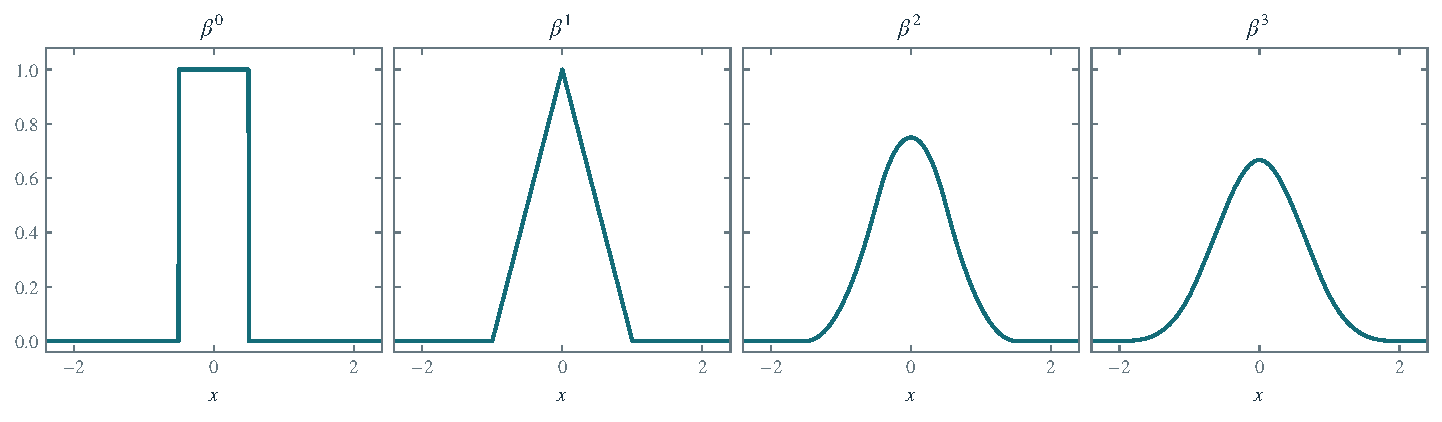
\includegraphics[width=1.0\linewidth]{figures/chapter-fourier-applications/centered-bsplines/figure.pdf}
\caption{Centered B-splines of degrees zero through three. Their support is $[-(n+1)/2,(n+1)/2]$.}
\label{fig-box-spline}
\end{figure}
\item Compute the continuous transform of $\beta^n$ and the periodic
transform $D_n=\widehat{\beta_d^n}$ of its integer samples.
For $n\geq1$, use Poisson summation without introducing an extra factor
$2\pi$. Prove $D_n>0$, separating even and odd values of $n+1$;
for odd powers, pair positive and negative frequency shifts and use an
alternating-series argument on $0\leq\xi\leq\pi$.
\item Define the cardinal kernel by
$\widehat{\beta^n_{\mathrm{card}}}(\xi)=\widehat{\beta^n}(\xi)/D_n(\xi)$.
Show $\beta^n_{\mathrm{card}}\to\sinc$ in $L^2(\RR)$, where
$\sinc(x)=\sin(\pi x)/(\pi x)$. One route is to write
$\xi=\eta+2\pi m$, $|\eta|\leq\pi$, and dominate the spectral tails by
$|\eta/(\eta+2\pi m)|^{n+1}$. Explain the connection with Shannon interpolation.
\begin{figure}[tbp]
\centering
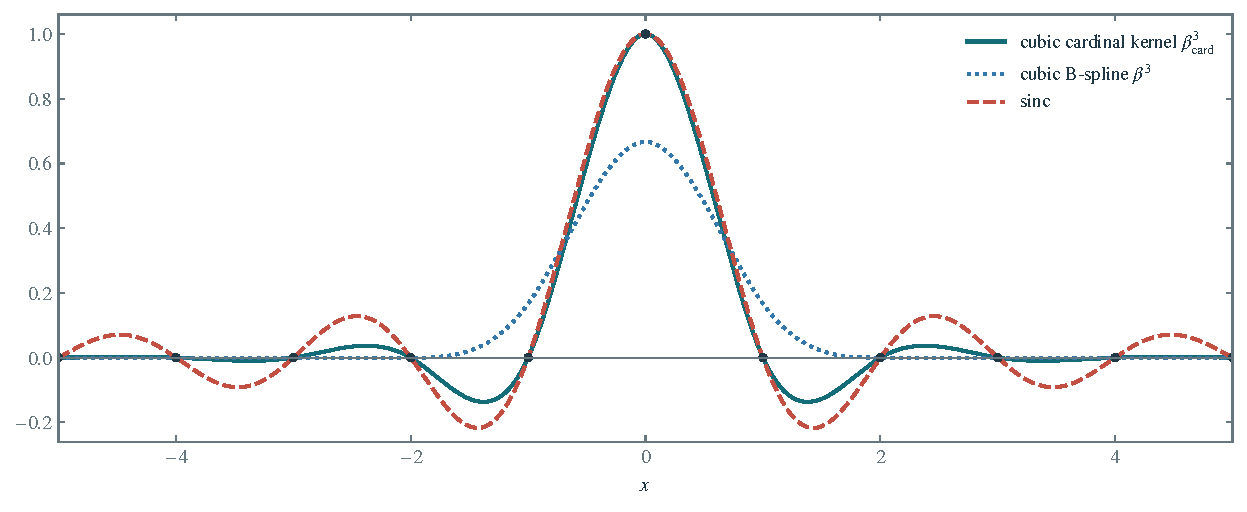
\includegraphics[width=1.0\linewidth]{figures/chapter-fourier-applications/cardinal-spline-and-sinc/figure.pdf}
\caption{The cubic cardinal kernel, the cubic B-spline, and sinc. The cardinal kernel and sinc equal one at zero and vanish at every other integer; the cubic B-spline requires a prefilter.}
\label{fig-comparison-spline-sinc}
\end{figure}
\item Explain how to approximate the prefilter by FFT for a finite sample
vector, and identify the boundary condition imposed by circular convolution.
Compare with recursive filtering in Exercise~\ref{exo-calcul-spline-iir}.
\end{enumerate}
For finitely many data points, boundary conditions select a unique cubic
spline. A \emph{natural} spline has zero \emph{second} derivative at both
endpoints; a spline with prescribed endpoint first derivatives is
\emph{clamped}. A \emph{not-a-knot} spline has continuous third derivative
at the first and last interior knots. Figure~\ref{fig-spline-cubic} compares
natural and not-a-knot conditions. See Ciarlet~\cite{ciarlet} and
Unser~\cite{unser-splines-perfect-fit} for complementary viewpoints.
\begin{figure}[tbp]
\centering
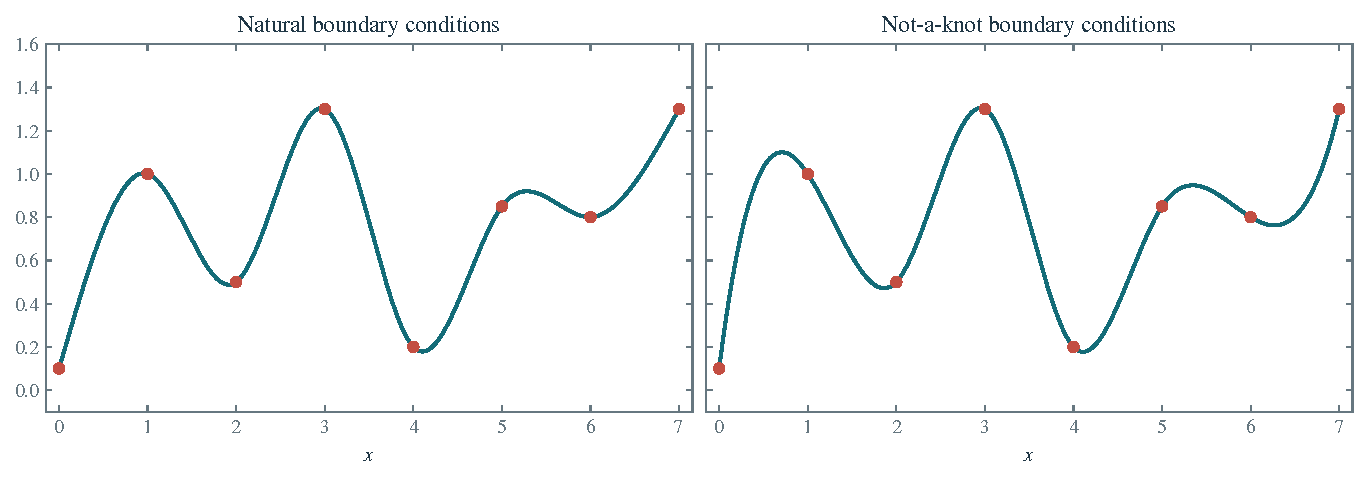
\includegraphics[width=1.0\linewidth]{figures/chapter-fourier-applications/cubic-spline-boundaries/figure.pdf}
\caption{Cubic interpolation of the same eight samples with natural and not-a-knot boundary conditions. Natural conditions set the endpoint second derivatives to zero.}
\label{fig-spline-cubic}
\end{figure}
\end{exo}

\section{Applications of the discrete Fourier transform}

\begin{correction}{exo-transforme-sup-comp}
Compact support and Cauchy--Schwarz give $\wh f\in L^1$. Fourier inversion
therefore defines a continuous representative. Differentiating under the
integral, with the bound $|\xi|^n\leq A^n$, gives
\[
 f^{(n)}(t_0)=\frac1{2\pi}\int_{-A}^A
             (\imath\xi)^n\wh f(\xi)e^{\imath\xi t_0}\d\xi.
\]
For every $z\in\CC$, the exponential series is dominated on this interval by
$e^{A|z-t_0|}|\wh f(\xi)|$, an integrable function. Thus
\[
 \frac1{2\pi}\int_{-A}^A\wh f(\xi)e^{\imath\xi z}\d\xi
 =\sum_{n=0}^\infty\frac{f^{(n)}(t_0)}{n!}(z-t_0)^n.
\]
This constructs an entire extension of $f$. If its real restriction vanishes
on an open interval, all derivatives at an interior point vanish, so the
series shows it is identically zero. If $f$ also has compact support,
its continuous representative vanishes outside that support and hence on an
open interval. Therefore $f=0$, proving the proposition.
\end{correction}

\begin{correction}{exo-resol-eq-heat-diff-finies}
\begin{enumerate}
\item Use the forward difference $(u(t+h,x)-u(t,x))/h$ in time and the
centered difference $(u(t,x+d)-2u(t,x)+u(t,x-d))/d^2$ in space.
The local consistency errors are $O(h)$ and $O(d^2)$ for smooth $u$.
\item The kernel is $g[0]=1-2s$, $g[\pm1]=s$. One direct step costs $O(N)$;
an FFT at every step would cost $O(N\log N)$. If only step $m$ is wanted,
two FFTs and the multipliers $\wh g[k]^m$ avoid computing all intermediate
steps. Program~\ref{listing-resolexplicite} implements the local stencil.
\begin{listing}[H]
\PythonCode{listing-resolexplicite}
\caption{Explicit heat evolution by a three-point stencil.}
\label{listing-resolexplicite}
\end{listing}
\item The multiplier is
\[
 r_k=1-4s\sin^2(\pi k/N).
\]
The DFT diagonalizes every power of the iteration. Boundedness for every
initial vector is equivalent to $|r_k|\leq1$ at every frequency, hence
$2s\mu_N\leq1$, where
\[
 \mu_N=\max_k\sin^2(\pi k/N)=
 \begin{cases}1,&N\text{ even},\\\cos^2(\pi/(2N)),&N\text{ odd}.\end{cases}
\]
This gives the stated bounds. The name CFL abbreviates
Courant--Friedrichs--Lewy. For $s\leq1/2$, the stencil is a convex average,
which also proves contraction in the maximum norm uniformly over grid sizes.
At the even-grid endpoint, the alternating mode has multiplier $-1$ and
remains bounded without decaying.
\item Write $a_k=-4s\sin^2(\pi k/N)\leq0$. The transformed equation gives
\[
 \wh u^{m+1}[k]=r_k\wh u^m[k],\qquad
 r_k=\frac{1+(1-\theta)a_k}{1-\theta a_k}.
\]
The denominator is positive, and $r_k\leq1$. The condition $r_k\geq-1$
is equivalent to $2+(1-2\theta)a_k\geq0$.
Thus the method is unconditionally stable for $\theta\geq1/2$.
For $\theta<1/2$, the exact fixed-grid condition is
$2s(1-2\theta)\mu_N\leq1$. The threshold is $1/2$, not $1/4$.
Program~\ref{listing-resolimplicite} evaluates any nonnegative integer
number of steps directly in Fourier coordinates.
\begin{listing}[H]
\PythonCode{listing-resolimplicite}
\caption{The one-dimensional theta method in Fourier coordinates.}
\label{listing-resolimplicite}
\end{listing}
\item On a square grid,
\[
 a_{kl}=-4s\bigl(\sin^2(\pi k/N)+\sin^2(\pi l/N)\bigr).
\]
For $\theta<1/2$, stability requires
$4s(1-2\theta)\mu_N\leq1$. In particular, the even-grid explicit bound
is $s\leq1/4$, not the one-dimensional bound $1/2$.
For $\theta\geq1/2$, stability is unconditional.
At $\theta=1/2$, $r_{kl}$ approaches $-1$ as $-a_{kl}$ grows:
high-frequency components alternate in sign while decaying very slowly.
At $\theta=1$, $r_{kl}=1/(1-a_{kl})$ approaches zero, so these components
are strongly damped. Program~\ref{listing-resolimplicite2d} implements both.
\begin{listing}[H]
\PythonCode{listing-resolimplicite2d}
\caption{The theta method on a periodic rectangular grid.}
\label{listing-resolimplicite2d}
\end{listing}
\end{enumerate}
\end{correction}

\begin{correction}{exo-unicite-eq-heat}
\begin{enumerate}
\item For $t>0$, absolute uniform convergence permits exchange of the integral
and the series:
\[
 p_t*f(x)=\sum_n e^{-2\pi^2n^2t}e^{2\pi\imath nx}
          \int_0^1f(y)e^{-2\pi\imath ny}\d y.
\]
On $t\geq\epsilon>0$, every differentiated series is dominated by a
polynomial in $|n|$ times $e^{-2\pi^2n^2\epsilon}$. Hence the convolution
is smooth and solves $u_t=\tfrac12u_{xx}$.
\item Two integrations by parts give $|c_n(f)|=O(|n|^{-2})$ for $n\ne0$.
Consequently,
\[
 \|u(t,\cdot)-f\|_\infty
 \leq\sum_n|c_n(f)|\,|e^{-2\pi^2n^2t}-1|\longrightarrow0
 \quad(t\downarrow0)
\]
by dominated convergence.
\item If $u(t_0,x_0)<0$, then $v=e^{\beta t}u$ attains a negative minimum
$\alpha$ on the compact cylinder $[0,t_0]\times S^1$.
Since the initial values are nonnegative, its minimizing time $t_1$ is
positive. At that point $v_{xx}\geq0$ and $v_t\leq0$; the latter also
holds at $t_1=t_0$ by the left derivative. But
$0\geq v_t=\beta\alpha+\tfrac12v_{xx}\geq\beta\alpha>0$
when $\beta<0$, a contradiction.
\item Apply positivity to smooth nonnegative initial functions, for which
continuity at $t=0$ was proved above. If $p_t$ were negative somewhere,
a nonnegative smooth bump supported near that point would give a negative
convolution value. Thus $p_t\geq0$. Its zeroth Fourier coefficient is one,
so its integral is one, and the integral triangle inequality gives
$\|p_t*f\|_\infty\leq\|f\|_\infty$.
For uniqueness, apply the minimum argument directly to $w$ and $-w$, where
$w$ is the difference of two real classical solutions with the same initial
values. Both have zero initial data, so $w=0$. For complex solutions apply
this to real and imaginary parts. This avoids assuming a representation
formula for an arbitrary solution.
\item Choose smooth periodic $f_j$ converging uniformly to $f$. Then
\[
 \|p_t*f-f\|_\infty
 \leq2\|f-f_j\|_\infty+\|p_t*f_j-f_j\|_\infty.
\]
First choose $j$ large, then let $t\downarrow0$. The first term is uniformly
small and the second tends to zero. This proves existence with the required
initial continuity, and the preceding maximum argument proves uniqueness.
\end{enumerate}
\end{correction}

\begin{correction}{exo-potential-electric-3d}
The stencil has coefficient $-6/h^2$ at the center and $1/h^2$ at each
of the six nearest neighbors. Each prescribed boundary neighbor is subtracted
from the right-hand side with factor $h^{-2}$. Odd extension in every
coordinate makes the boundary values zero and yields a $2N$-periodic array.
Its symbol is
\[
 -\frac4{h^2}\left(\sin^2\frac{\pi k}{2N}
                  +\sin^2\frac{\pi l}{2N}
                  +\sin^2\frac{\pi m}{2N}\right).
\]
Divide the transformed right-hand side by this symbol away from zero and
set the zero coefficient to zero. Invert the transform, retain the interior,
and restore the prescribed boundary. Program~\ref{listing-antisymmetrise}
constructs the odd extension in any dimension. The general solver in
Program~\ref{fish-listing} likewise works in two or three dimensions.
\begin{listing}[H]
\PythonCode{listing-antisymmetrise}
\caption{Odd extension along every coordinate axis.}
\label{listing-antisymmetrise}
\end{listing}
\end{correction}

\begin{correction}{exo-formulation-matrix-fish}
\begin{enumerate}
\item Multiplication by $T$ on the left takes second differences in the first
index; multiplication on the right takes them in the second. Their sum is
the five-point stencil with zero boundary values.
\item A boundary value is a known contribution to that stencil, so move it
to the right with coefficient $-h^{-2}$. Summing the contributions at corners
of the interior grid gives precisely $\wt F$ in the main text.
\item With $V_j[i]=\sin(\pi ij/N)$ and zero values at $i=0,N$,
\[
 (TV_j)[i]=\lambda_jV_j[i],\qquad
 \lambda_j=-4h^{-2}\sin^2(\pi j/(2N)).
\]
These eigenvalues are negative and distinct for $1\leq j<N$.
Let $U_0=V^{-1}\wt UV$ and $F_0=V^{-1}\wt FV$. Then
$(\lambda_i+\lambda_j)(U_0)_{ij}=(F_0)_{ij}$, so division determines
$U_0$ uniquely; no denominator vanishes. Finally $\wt U=VU_0V^{-1}$.
\item Symmetry of $T$ gives orthogonality between distinct eigenvectors,
and the identity $\sum_{i=1}^{N-1}\sin^2(\pi ij/N)=N/2$ gives
$V^TV=(N/2)I$. Since $V=V^T$, its inverse is $(2/N)V$.
Thus $V$ is \emph{scaled orthogonal}; $Q=\sqrt{2/N}V$ is orthogonal.
The product $Vx$ is the unnormalized sine transform $\Ss x$.
\item For the length-$2N$ odd extension
$x^o=(0,x[1],\ldots,x[N-1],0,-x[N-1],\ldots,-x[1])$,
\[
 \widehat{x^o}[k]
 =\sum_{j=1}^{N-1}x[j](e^{-\pi\imath jk/N}-e^{\pi\imath jk/N})
 =-2\imath\Ss(x)[k].
\]
Hence $\Ss x=\widehat{x^o}[1:N]/(-2\imath)$ and
$\Ss^{-1}=(2/N)\Ss$. The identity holds for complex data as well; taking
an imaginary part alone would discard information in that case.
Program~\ref{listing-transfo-sinus} preserves complex input.
\begin{listing}[H]
\PythonCode{listing-transfo-sinus}
\caption{The unnormalized sine transform, preserving complex data.}
\label{listing-transfo-sinus}
\end{listing}
For an interior matrix $F$, applying the transform in both coordinates gives
$\Ss_2(F)=VFV$, with inverse $(2/N)^2\Ss_2$.
The doubled odd array satisfies
$\widehat{F^o}[k,l]=-4(VFV)_{kl}$ on the interior frequencies.
Thus both constructions divide by the same eigenvalue sums and reconstruct
the same solution. Program~\ref{listing-transfo-sinus-2d} applies the
one-dimensional transform along the two axes.
\begin{listing}[H]
\PythonCode{listing-transfo-sinus-2d}
\caption{A two-dimensional sine transform.}
\label{listing-transfo-sinus-2d}
\end{listing}
\end{enumerate}
\end{correction}

\begin{correction}{exo-lissage-image}
Program~\ref{listing-calculfiltre} samples a Gaussian and normalizes its
finite sum to one. Its default radius is $\lceil4\sigma\rceil$ pixels.
Program~\ref{listing-appliquefiltre} reads a grayscale image and convolves
a reflected extension with this kernel, retaining the valid output.
Reflection preserves constant images and avoids an artificial dark border.
The noise is reduced at the cost of some edge and texture detail.
\begin{listing}[H]
\PythonCode{listing-calculfiltre}
\caption{A finite Gaussian kernel with unit sum.}
\label{listing-calculfiltre}
\end{listing}
\begin{listing}[H]
\PythonCode{listing-appliquefiltre}
\caption{Gaussian image smoothing with reflected boundaries.}
\label{listing-appliquefiltre}
\end{listing}
\end{correction}

\begin{correction}{exo-correlation-2d}
\begin{enumerate}
\item Expanding the square gives
\[
 d(f,g)[u,v]^2=E_f[u,v]+\|g\|_2^2-2\Corr(f,g)[u,v].
\]
If $E_f$ is constant, minimizing the squared discrepancy is exactly equivalent
to \emph{maximizing} correlation. If it varies little, this is only an approximation.
Full-template positions are essential here: otherwise the norm of the
visible part of $g$ also depends on the position.
\item Let $\check g[i,j]=g[-i,-j]$, with zero extension. Then
$\Corr(f,g)[u,v]=(f\star\check g)[u,v]$.
When the reflected template is stored as the ordinary array
$g[P-1-i,P-1-j]$, the corresponding full-convolution indices are
$(u+P-1,v+P-1)$. Padding to at least $N+P-1$ in both coordinates avoids
wraparound; extracting the valid part gives all complete-template positions.
\item Center the patch and template, writing their vectorized forms as
$a$ and $b$. For nonzero $a,b$,
$\rho=\langle a,b\rangle/(\|a\|_2\|b\|_2)$.
Cauchy--Schwarz gives $|\rho|\leq1$; equality $\rho=1$ means
$a=cb$ for some $c>0$, not necessarily $a=b$.
Offsets and positive rescalings of either intensity leave $\rho$ unchanged;
a negative rescaling of one image reverses its sign. A constant template
or patch has zero variance, so normalized correlation is undefined there.
\item Since $g_0=g-\mu_g$ has zero sum, the numerator is
$\sum_{i,j}f[u+i,v+j]g_0[i,j]$. This is one FFT-based correlation.
The patch variance is $s_2-s_1^2/P^2$, and the template variance
$\sum_{i,j}g_0[i,j]^2$ is computed once.
The stated recurrence follows by inclusion--exclusion of four overlapping
windows; the four corner terms must all contain the power $k$.
A summed-area table gives the equivalent formula
\[
 s_k[u,v]=I_k[u+P,v+P]-I_k[u,v+P]-I_k[u+P,v]+I_k[u,v],
\]
where $I_k[a,b]=\sum_{i<a,j<b}f[i,j]^k$.
Two cumulative sums construct $I_k$ in $O(N^2)$ work, after which each
window costs four lookups. Program~\ref{sliding-sum-listing} implements this.
\begin{listing}[H]
\PythonCode{sliding-sum-listing}
\caption{Sliding sums from a summed-area table.}
\label{sliding-sum-listing}
\end{listing}
Program~\ref{listing-correlation-normalized} combines these sums with FFT
correlation, for total cost $O(N^2\log N)$. It uses the Frobenius norm of
the template, subtracts a global image offset to reduce cancellation, and
marks zero-variance patches with \texttt{NaN}. Tiny negative computed
variances are clipped to zero before square roots; this corrects roundoff,
not the mathematical definition.
\begin{listing}[H]
\PythonCode{listing-correlation-normalized}
\caption{Normalized correlation at complete-template positions.}
\label{listing-correlation-normalized}
\end{listing}
\end{enumerate}
\end{correction}

\begin{correction}{exo-fft-rotation}
\begin{enumerate}
\item For signed frequencies $k,l$,
\[
 \widehat{T_vf}[k,l]=e^{-2\pi\imath(kv_1+lv_2)/N}\wh f[k,l].
\]
For integer shifts, this follows by changing indices. For fractional shifts,
it defines translation of the chosen trigonometric interpolant. Using
unsigned frequencies instead would select a different interpolation between
samples. Odd sizes avoid the unmatched real Nyquist mode of even sizes.
Program~\ref{listing-ffttranslation} implements the formula.
\begin{listing}[H]
\PythonCode{listing-ffttranslation}
\caption{Fractional translation using signed Fourier frequencies.}
\label{listing-ffttranslation}
\end{listing}
For an $x$-shear, translate each fixed-$y$ column by $\lambda y$; for a
$y$-shear, translate each fixed-$x$ row by $\lambda x$. Centered coordinates
place the center of the image at the origin.
Program~\ref{listing-ffttransvec} implements either axis.
\begin{listing}[H]
\PythonCode{listing-ffttransvec}
\caption{A centered shear along either image coordinate.}
\label{listing-ffttransvec}
\end{listing}
\item Multiply the three matrices with
$a=-\tan(\theta/2)$ and $b=\sin\theta$. The diagonal entries are
$1+ab=\cos\theta$, the lower-left entry is $b$, and the upper-right entry
is $2a+a^2b=-\sin\theta$. Since pullbacks compose in the corresponding
matrix order,
$R_\theta=S_a^{(x)}S_b^{(y)}S_a^{(x)}$ for continuous functions.
\item Each discrete line translation is unitarily diagonalized by the DFT,
with unit-modulus multipliers. Its inverse negates the shift, so each shear
and their product are invertible. Reversing the three steps and negating
their parameters gives the inverse; the symmetric three-step pattern makes
it the algorithm with angle $-\theta$.
\begin{listing}[H]
\PythonCode{listing-fftrotation}
\caption{Rotation by three discrete shears.}
\label{listing-fftrotation}
\end{listing}
Nevertheless, intermediate sheared functions do not generally belong to
the original finite tensor-product trigonometric space. Resampling and
periodic wrapping therefore prevent these discrete matrices from forming
an exact representation of all planar rotations:
$R_\alpha R_\beta\ne R_{\alpha+\beta}$ in general.
Taking real parts on even grids or cropping intermediate results can also
destroy invertibility. The odd-grid implementation preserves real data
without discarding a Nyquist component, and preserves complex data as complex.

Padding moves wraparound away from the image of interest; it does not make
band-limited interpolation exact for arbitrary continuous images.
Program~\ref{listing-applies-rotation} supplies a white margin for a small
rotation gallery. Larger angles should be split into bounded steps or
reduced using quarter-turn permutations to avoid very large shears.
The arithmetic cost is $O(N^2\log N)$ for a square padded grid.
\begin{listing}[H]
\PythonCode{listing-applies-rotation}
\caption{A rotation gallery with a padded white margin.}
\label{listing-applies-rotation}
\end{listing}
\end{enumerate}
\end{correction}

\begin{correction}{exo-creation-low-pass-filter}
\begin{enumerate}
\item Form the real even sampled response $H[k]=\mathbf1_{|\omega_k|<\pi/2}$,
with half-values at any cutoff samples, and take its inverse DFT.
The resulting circular kernel is real and symmetric, and its sum is $H[0]=1$.
\begin{listing}[H]
\PythonCode{listing-low-pass-filter}
\caption{A sharp sampled low-pass response and its inverse transform.}
\label{listing-low-pass-filter}
\end{listing}
\item Assign kernel indices to $-(N-1)/2,\ldots,(N-1)/2$, then embed them
modulo a larger plotting length. Padding the negative-index terms at the
wrong end would change the response. The resulting FFT samples
$G(\omega)=\sum_jg[j]e^{-\imath j\omega}$, which agrees with $H$ at the
original frequencies but oscillates between them near the cutoff.
Program~\ref{listing-drawing-filter-zero-padding} returns the frequencies
and the complex response; for this symmetric real kernel it is real up to roundoff.
\begin{listing}[H]
\PythonCode{listing-drawing-filter-zero-padding}
\caption{Dense frequency-response evaluation with centered kernel indices.}
\label{listing-drawing-filter-zero-padding}
\end{listing}
\item Let $r=|\omega|$, $a=(1-\epsilon)\pi/2$, and
$b=(1+\epsilon)\pi/2$. Use response one for $r\leq a$, zero for $r\geq b$,
and $\tfrac12[1+\cos(\pi(r-a)/(b-a))]$ in the transition.
At $\epsilon=0$ use the sharp-cutoff definition separately.
Increasing the transition width reduces the long oscillatory tails of the
impulse response. The endpoint $\epsilon=1$ is included without creating
a negative array length.
\begin{listing}[H]
\PythonCode{configurable-filter-listing}
\caption{A raised-cosine transition, including both endpoint parameters.}
\label{configurable-filter-listing}
\end{listing}
\end{enumerate}
\end{correction}

\begin{correction}{exo-iterations-integers}
\begin{enumerate}
\item The rounded update is
$a_j^{m+1}=2\lceil(a_j^m+a_{j-1}^m)/4\rceil$.
Its minimum is nondecreasing and its maximum nonincreasing, since both are
even. If the current minimum is $q$, an updated count equals $q$ exactly
when both contributing counts equal $q$. Thus its new minimum set is the
intersection of the old minimum set and its one-step translate.
A nonempty proper subset of a cycle cannot be invariant under a one-step
translation, so its cardinality strictly decreases while the minimum stays
fixed. Within at most $n$ steps, either consensus is reached or the minimum
increases by at least two. It is bounded above by the initial maximum,
so consensus occurs after finitely many steps. This argument excludes the
already-constant case before claiming strict decrease.
\item Without rounding, the kernel is $(1/2,1/2,0,\ldots,0)$.
Its nonconstant Fourier multipliers have modulus less than one, so the limit
is the constant vector with value $n^{-1}\sum_ja_j^0$.
\item With half sent to each neighbor, the multiplier is
$\cos(2\pi k/n)$. For odd $n$, its modulus is less than one except at zero,
so the fractional process converges to the mean. For even $n$, the
alternating mode has multiplier $-1$: alternating counts $0,2,0,2,\ldots$
are exchanged at every step and do not converge, even with rounding.
For the rounded process on an odd cycle, a site remains at the current
minimum exactly when both its neighbors were at that minimum.
If the minimum set failed to shrink, it would be invariant under translation
by two. Since two generates an odd cycle, a proper nonempty minimum set
cannot have this property. The preceding finite-consensus argument therefore
applies to odd $n$ as well.
\end{enumerate}
\end{correction}

\begin{correction}{exo-algo-karatsuba}
\begin{enumerate}
\item The terms are $R_0=P_0Q_0$, $R_2=P_1Q_1$, and
$R_1=P_0Q_1+P_1Q_0$.
\item Compute
$R_1=(P_0+P_1)(Q_0+Q_1)-R_0-R_2$.
The cross term needs one new product, two additions, and two subtractions.
\item After padding to length $n=2^p$, the recurrence is
$C(n)=3C(n/2)+O(n)$, hence
\[
 C(n)=O\!\left(\sum_{j=0}^{p-1}3^j\frac n{2^j}+3^p\right)
     =O(n^{\log_2 3}).
\]
Padding arbitrary lengths increases them by less than a factor two and
preserves the bound. Programs~\ref{listing-karatsuba} and \ref{listing-add}
use Python lists, so integer coefficients retain arbitrary precision.
The algebra also works over other coefficient rings supporting addition,
subtraction, and multiplication. There is no universal crossover degree:
benchmark comparable implementations and include conversion and precision costs.
\begin{listing}[H]
\PythonCode{listing-karatsuba}
\caption{Karatsuba multiplication with exact Python integer coefficients.}
\label{listing-karatsuba}
\end{listing}
\begin{listing}[H]
\PythonCode{listing-add}
\caption{Addition of coefficient vectors of different lengths.}
\label{listing-add}
\end{listing}
\end{enumerate}
\end{correction}

\begin{correction}{exo-spline-filtering}
\begin{enumerate}
\item The interpolation equations are $u_d=a*\psi_d$.
Since $\psi_d$ is finitely supported, its transform $D=\widehat{\psi_d}$
is continuous and periodic. Nonvanishing therefore implies
$\min_{[-\pi,\pi]}|D|>0$, so multiplication by $D$ is a boundedly
invertible operator on $L^2$ of the circle. This proves the unique solution
$\widehat a=\widehat{u_d}/D$.
Let $b$ have Fourier series $1/D$ and set
$\varphi(x)=\sum_kb[k]\psi(x-k)$. At each $x$, this sum has finitely many
nonzero terms; moreover $b*\psi_d=\delta_0$, so $\varphi(j)=\delta_{j0}$.
Then $a=b*u_d$ gives the direct form with kernel $\varphi$.
The inverse filter generally has infinitely many coefficients, so compact
support of $\psi$ need not imply compact support of $\varphi$.
\item Repeated convolution gives
$\Supp(\beta^n)=[-(n+1)/2,(n+1)/2]$ (as a closed support).
Direct interpolation requires $\beta^n(j)=\delta_{j0}$.
This holds for $n=0$ and $n=1$, giving piecewise constant and piecewise linear
interpolation. It fails for $n\geq2$; these degrees require a prefilter.
\item Put $r=n+1$. The continuous convolution theorem gives
\[
 B_r(\xi):=\widehat{\beta^n}(\xi)
          =\left(\frac{\sin(\xi/2)}{\xi/2}\right)^r.
\]
For $n\geq1$, Poisson summation, with absolutely convergent frequency tails,
gives
\[
 D_n(\xi)=\sum_{k\in\ZZ}\beta^n(k)e^{-\imath k\xi}
         =\sum_{m\in\ZZ}B_r(\xi+2\pi m).
\]
There is no factor $2\pi$ in this identity. By evenness and periodicity it
suffices to take $0\leq\xi\leq\pi$.
If $r$ is even, every summand is nonnegative and $B_r(\xi)>0$.
If $r\geq3$ is odd, put $x=\xi/(2\pi)$. For $0<x\leq1/2$, pairing the
terms $m=j$ and $m=-j$ gives
\[
 D_n(\xi)=B_r(\xi)+\left(\frac{\sin(\pi x)}\pi\right)^r
 \sum_{j=1}^\infty(-1)^{j+1}
       \left((j-x)^{-r}-(j+x)^{-r}\right).
\]
The parenthesized quantities are positive and decrease to zero: their
derivative as a function of $j$ is negative. The alternating sum is
nonnegative. Thus in both parity cases
$D_n(\xi)\geq B_r(\xi)>0$ on $[-\pi,\pi]$; at zero both sides equal one.
For $n=0$, the sampled sequence is simply $\delta_0$, so $D_0=1$.
\item The transform of the cardinal kernel is $H_r=B_r/D_n$.
For $|\eta|\leq\pi$ and $m\in\ZZ$,
\[
 |H_r(\eta+2\pi m)|
 \leq\left|\frac{\eta}{\eta+2\pi m}\right|^r,
\]
with the $m=0$ ratio interpreted as one. This follows from
$D_n(\eta)\geq B_r(\eta)>0$ and the ratio of the two sinc powers.
For $|\eta|<\pi$, every ratio with $m\ne0$ is strictly less than one, and
the shifted series shows $D_n(\eta)/B_r(\eta)\to1$ as $r\to\infty$.
Consequently $H_r(\eta)\to1$ and $H_r(\eta+2\pi m)\to0$ for $m\ne0$,
except at a set of endpoints of measure zero.

For $r\geq2$ and $m\ne0$, the squared terms are bounded by
$(2|m|-1)^{-4}$. This bound is summable in $m$ and integrable over
$\eta\in[-\pi,\pi]$, while $|H_r(\eta)|\leq1$ on the central interval.
Dominated convergence on these intervals therefore proves
$H_r\to\mathbf1_{[-\pi,\pi]}$ in $L^2(\RR)$.
Since $\widehat{\sinc}=\mathbf1_{[-\pi,\pi]}$ in our convention,
Plancherel gives $\beta^n_{\mathrm{card}}\to\sinc$ in $L^2$.
The argument keeps the alternating signs for even spline degrees; dropping
them would give a different cardinal kernel.

For the cubic spline, $D_3(\xi)=(2+\cos\xi)/3$ and its inverse filter is
$b[k]=\sqrt3(\sqrt3-2)^{|k|}$. Hence
\[
 \beta^3_{\mathrm{card}}(x)=\sqrt3\sum_{k\in\ZZ}
              (\sqrt3-2)^{|k|}\beta^3(x-k).
\]
It has unbounded, exponentially decaying tails, whereas sinc decays only
algebraically. The limiting cardinal interpolation uses sinc translates,
as in Shannon's sampling theorem.
\item For a finite vector, division by sampled values of $D_n$ followed by
an inverse FFT computes the \emph{periodic} prefilter exactly for that finite
model. It approximates the infinite-grid problem only after a boundary model
and sufficient extension have been chosen. The principal issue is the
unintended periodic boundary condition, rather than an unavoidable failure
of FFT convolution. Recursive causal and anticausal filters exploit the
roots of the spline symbol; Exercise~\ref{exo-calcul-spline-iir} develops
this method for cubic splines. Natural and not-a-knot finite-interval splines
solve different boundary-value problems and should not be conflated with
periodic or infinite-grid interpolation.
\end{enumerate}
\end{correction}

